% ============================================================
%  Claude X-Ray — IEEE Conference Format
%  Static Analysis of claw-code (Python port of Claude Code)
%  Author: Diego Díaz Montero — April 2026
% ============================================================

\documentclass[conference]{IEEEtran}

% ---------------------------------------------------------------
% Packages
% ---------------------------------------------------------------
\usepackage[T1]{fontenc}
\usepackage[utf8]{inputenc}
\usepackage{microtype}

\usepackage{graphicx}
\graphicspath{{graphs/}}

\usepackage{amsmath}
\usepackage{amssymb}
\usepackage{booktabs}
\usepackage{multirow}
\usepackage{array}
\usepackage{url}
\usepackage{cite}
\usepackage{xcolor}
\usepackage{listings}
\usepackage{algorithm}
\usepackage{algorithmic}
\usepackage{balance}
\usepackage{hyperref}

% ---------------------------------------------------------------
% Listings style
% ---------------------------------------------------------------
\lstset{
  basicstyle=\scriptsize\ttfamily,
  breaklines=true,
  breakatwhitespace=false,
  frame=single,
  captionpos=b,
  keywordstyle=\color{blue!80!black},
  commentstyle=\color{gray!70},
  stringstyle=\color{red!65!black},
  numbers=left,
  numberstyle=\tiny\color{gray},
  numbersep=5pt,
  xleftmargin=10pt,
  aboveskip=4pt,
  belowskip=4pt,
  showstringspaces=false
}

% ---------------------------------------------------------------
% Hyperref
% ---------------------------------------------------------------
\hypersetup{
  colorlinks=true,
  linkcolor=blue!70!black,
  citecolor=blue!70!black,
  urlcolor=blue!70!black
}

% ---------------------------------------------------------------
\begin{document}
% ---------------------------------------------------------------

\title{Claude X-Ray: Reverse-Engineering the Internal Architecture\\
of an LLM-Powered Agentic CLI via Static Analysis}

\author{
  \IEEEauthorblockN{Diego D{\'i}az Montero}
  \IEEEauthorblockA{
    Data Science Student \\
    Static Analysis of \texttt{claw-code} ---
    Python Port of Claude Code \\
    April 2026
  }
}

\maketitle

% ---------------------------------------------------------------
\begin{abstract}
Large Language Model (LLM) agentic systems are increasingly deployed
as developer tools, yet their internal architectures remain opaque ---
making it difficult to reason about reliability, memory behavior, and
architectural coupling. This paper presents \emph{Claude X-Ray}, a
systematic static analysis of \texttt{claw-code}, the open Python port
of Anthropic's Claude Code agentic CLI. We apply import-graph analysis,
the PageRank centrality algorithm, DAG-based longest-path computation,
AST string extraction, and pattern-matching for feature flags to expose
the full internal architecture of an otherwise closed-source production
AI agent. Our analysis covers 1,902 TypeScript source files compiled
into 66 Python modules, 207 slash commands, 184 registered tools, and
29 subsystems. We identify a critical architectural bottleneck (15\% of
all import-graph traffic concentrated through three files), pinpoint the
exact line of code where Claude forgets old conversation turns
(\texttt{compact(keep\_last=10)}), reconstruct a 7-stage bootstrap
pipeline that fires before every invocation, and discover a sparse
feature-flag surface of only 4 toggles across the entire system. Our
findings have direct implications for developers building on top of
Claude Code and for the broader LLM agent engineering community.
\end{abstract}

\begin{IEEEkeywords}
LLM agents, static analysis, software architecture, dependency graphs,
PageRank, Claude Code, AI tooling, memory management, reverse engineering.
\end{IEEEkeywords}

% ---------------------------------------------------------------
\section{Introduction}
% ---------------------------------------------------------------

\IEEEPARstart{T}{he} emergence of LLM agentic systems has introduced
a new class of software infrastructure: persistent, tool-augmented AI
processes that interleave code execution, file manipulation, and
multi-turn dialogue to complete engineering tasks
autonomously~\cite{yao2022react,shinn2023reflexion}. Anthropic's
Claude Code~\cite{anthropic2024claudecode} is among the most prominent
such systems, serving as an official agentic CLI for software
development. Despite its widespread use, Claude Code's internal
architecture is closed source, leaving practitioners without visibility
into its dependency structure, initialization pipeline, memory
management, or feature-flag surface.

Understanding these internals matters for several reasons. First,
architectural bottlenecks in critical files cascade into system-wide
failures. Second, memory eviction policies determine observable
conversation behavior. Third, initialization pipeline failures are
often misdiagnosed by end users. Fourth, feature-flag sparsity limits
the degree to which the system can be configured or extended.

This paper presents \emph{Claude X-Ray}, a static analysis study of
\texttt{claw-code}~\cite{instructkr2024clawcode}, the open Python port
of Claude Code's agent harness compiled from the original TypeScript
implementation. Using a combination of graph-theoretic, AST-based, and
pattern-matching techniques, we reconstruct the hidden architecture of
Claude Code entirely through program analysis --- no runtime
instrumentation required.

\subsection{Contributions}

This work makes the following contributions:

\begin{enumerate}
  \item A \textbf{full dependency graph} of 66 Python modules with
        PageRank centrality scores, identifying the 10 most architecturally
        critical files.

  \item Identification of a \textbf{critical import concentration}: 15\%
        of the entire import graph flows through exactly 3 files
        (\texttt{models} $\to$ \texttt{commands} $\to$ \texttt{tools}).

  \item Discovery of \textbf{Claude's memory eviction mechanism}: the
        \texttt{compact(keep\_last=10)} call in \texttt{transcript.py}
        is the precise location where conversation history is truncated.

  \item Reconstruction of the \textbf{7-stage bootstrap pipeline} that
        executes before every agent invocation.

  \item A \textbf{feature-flag audit} revealing only 4 boolean flags
        across the entire system, all on by default.
\end{enumerate}

% ---------------------------------------------------------------
\section{Background and Related Work}
% ---------------------------------------------------------------

\subsection{LLM Agentic Systems}

ReAct~\cite{yao2022react} introduced the paradigm of interleaving
reasoning and acting in LLM agents. Subsequent systems such as
AutoGPT~\cite{significantgravitas2023autogpt}, LangChain
Agents~\cite{langchain2023}, and Claude Code generalize this pattern
into production-grade tooling. The shared architectural elements
include a tool registry, a task/query router, session memory, and
a command dispatch layer --- all of which we identify and characterize
in this paper.

\subsection{Static Analysis of AI Systems}

Prior work has applied static analysis to neural network
code~\cite{zhang2020static} and to safety audits of LLM
prompts~\cite{perez2022ignore}, but systematic program analysis of
full LLM agent harnesses remains underexplored. Our work bridges this
gap by applying classical software analysis (PageRank on import graphs,
DAG longest-path, AST mining) to an LLM agent codebase.

\subsection{Dependency Graph Analysis}

PageRank~\cite{page1999pagerank} was originally designed for web-link
graphs but has been applied extensively to software dependency
graphs~\cite{bavota2014mining} to identify architecturally critical
modules. We apply it here to the Python module import graph of
\texttt{claw-code}.

% ---------------------------------------------------------------
\section{Data and Methodology}
% ---------------------------------------------------------------

\subsection{Data Source}

Our primary artifact is \texttt{claw-code}~\cite{instructkr2024clawcode},
an open Python port of Claude Code's TypeScript agent harness. The
dataset comprises 66 Python source modules, 1,902 original TypeScript
source files (archived), 207 slash commands, 184 registered tools, and
29 subsystems. Reference snapshots (JSON) were parsed for metadata
enrichment. All analysis is purely static --- no runtime execution was
performed.

\subsection{Import Graph Construction}

We parse each Python module's \texttt{import} and
\texttt{from...import} statements using Python's \texttt{ast} module
to construct a directed graph $G = (V, E)$, where $V$ is the set of
modules and $E$ represents import dependencies.

\subsection{PageRank Centrality}

PageRank~\cite{page1999pagerank} is computed on $G$ to quantify the
influence of each module. For module $v$:

\begin{equation}
  PR(v) = \frac{1-d}{|V|} + d \sum_{u \in \mathrm{in}(v)}
  \frac{PR(u)}{|\mathrm{out}(u)|}
  \label{eq:pagerank}
\end{equation}

where $d = 0.85$ is the damping factor, $\mathrm{in}(v)$ is the set
of modules that import $v$, and $|\mathrm{out}(u)|$ is the number of
modules imported by $u$.

\subsection{Longest Dependency Chain}

We compute the longest path in the DAG (after cycle removal) using
topological sorting. This gives the maximum transitive dependency depth
and serves as a proxy for architectural coupling.

\subsection{AST String Extraction}

We extract all string constants $\geq 40$ characters from module ASTs,
revealing hardcoded instructions, behavioral directives, and internal
labels embedded in Claude Code's source.

\subsection{Feature Flag Detection}

We apply keyword pattern matching to identify boolean variables
containing terms: \texttt{enable}, \texttt{mode}, \texttt{hook},
\texttt{mcp}, \texttt{skill}. For each match we record the file,
line number, flag name, and default value.

% ---------------------------------------------------------------
\section{Results}
% ---------------------------------------------------------------

\subsection{Dependency Graph Overview}

The import graph $G$ has $|V| = 66$ nodes and $|E| = 57$ directed
edges. The graph is sparse relative to its node count, with an average
out-degree of 0.86, suggesting deliberate modularization. Figure
\ref{fig:dep_graph} shows the full dependency network.

\begin{figure}[!t]
  \centering
  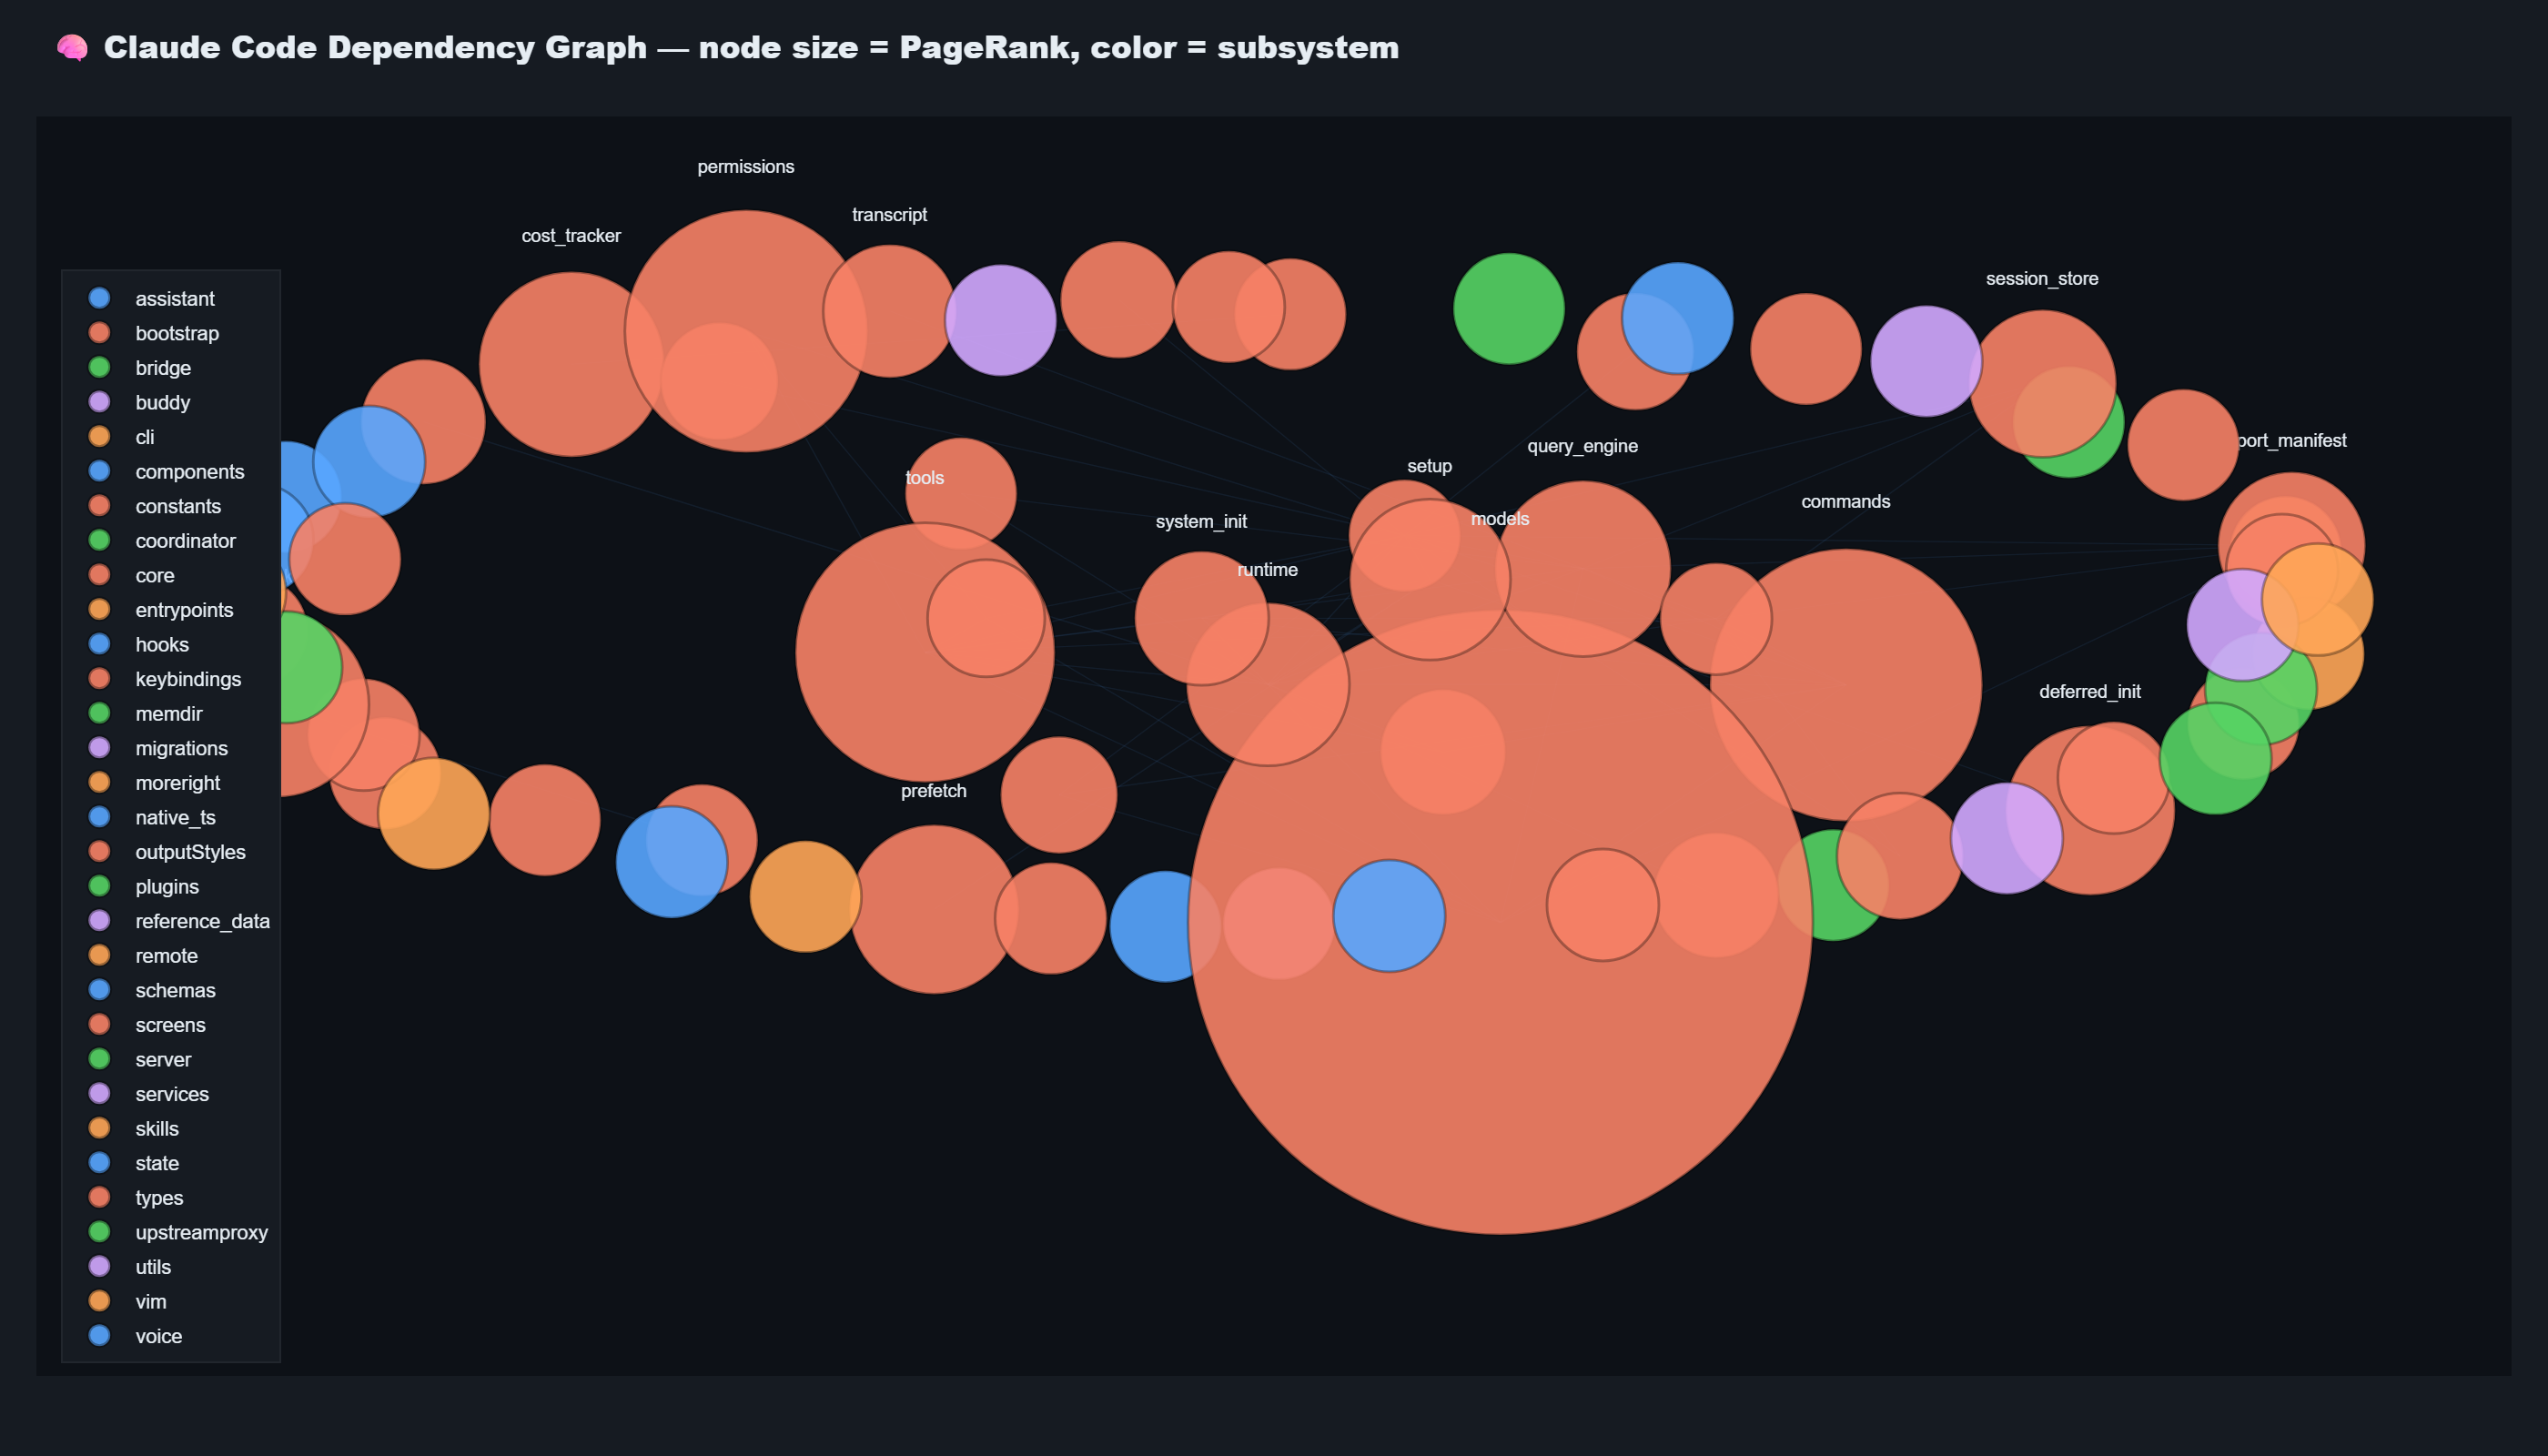
\includegraphics[width=\columnwidth]{01_dependency_graph.png}
  \caption{Full import dependency graph of Claude Code (66 Python
    modules). Node size $\propto$ PageRank centrality; color encodes
    subsystem cluster. The \texttt{models}$\to$\texttt{commands}$\to$%
    \texttt{tools} bottleneck is visually prominent at the center.}
  \label{fig:dep_graph}
\end{figure}

\subsection{PageRank: Critical Files}

Table~\ref{tab:pagerank} lists the top 10 modules by PageRank score.
Figure~\ref{fig:pagerank} visualizes the score distribution.

\begin{table}[!t]
  \renewcommand{\arraystretch}{1.25}
  \caption{Top 10 Modules by PageRank Centrality}
  \label{tab:pagerank}
  \centering
  \resizebox{\columnwidth}{!}{%
  \begin{tabular}{@{}clcl@{}}
    \toprule
    \textbf{Rk} & \textbf{Module} & \textbf{Sub.} & \textbf{Role} \\
    \midrule
    1  & \texttt{query\_engine}  & core   & Central router    \\
    2  & \texttt{runtime}        & core   & Runtime manager   \\
    3  & \texttt{deferred\_init} & core   & Lazy initializer  \\
    4  & \texttt{prefetch}       & core   & Resource pre-load \\
    5  & \texttt{cost\_tracker}  & core   & Token accounting  \\
    6  & \texttt{task}           & core   & Task lifecycle    \\
    7  & \texttt{permissions}    & core   & Access control    \\
    8  & \texttt{session\_store} & memdir & Session persist.  \\
    9  & \texttt{transcript}     & memdir & In-memory turns   \\
    10 & \texttt{history}        & state  & Event log         \\
    \bottomrule
  \end{tabular}}
\end{table}

\begin{figure}[!t]
  \centering
  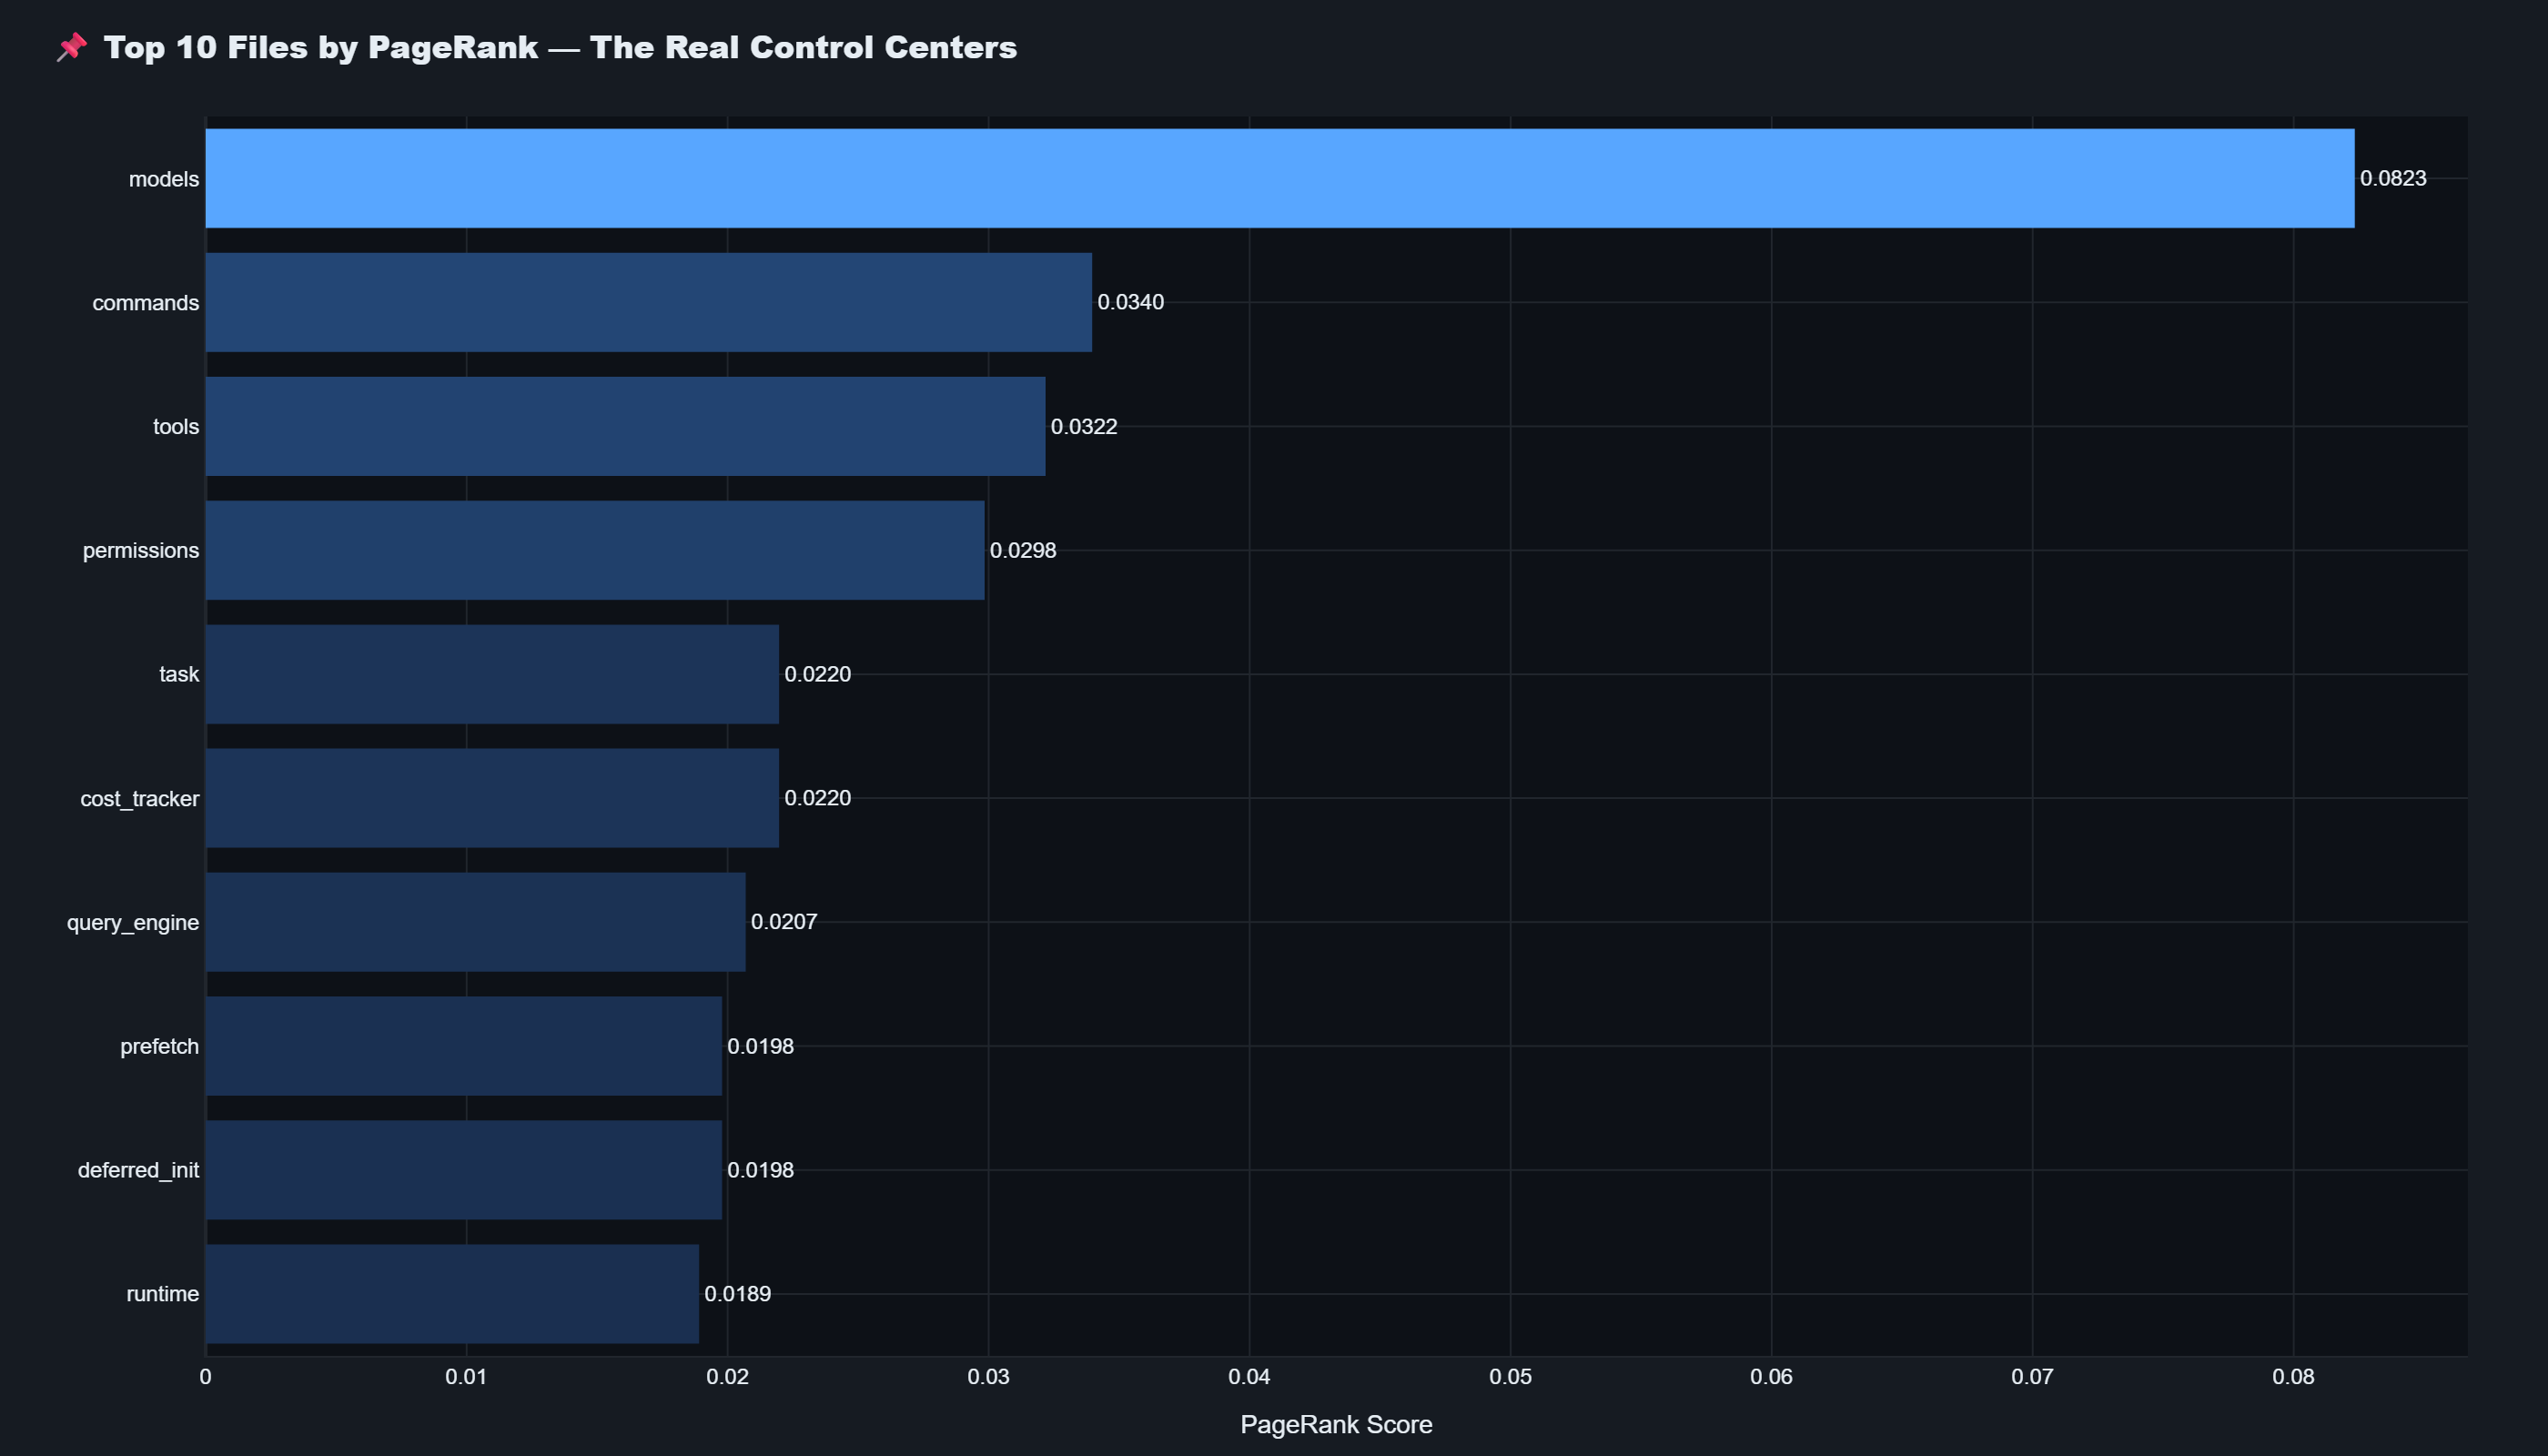
\includegraphics[width=\columnwidth]{03_pagerank_top10.png}
  \caption{Top 10 modules ranked by PageRank centrality.
    \texttt{query\_engine} leads by a significant margin, confirming
    its role as the architectural center of the system.}
  \label{fig:pagerank}
\end{figure}

\subsection{Import Concentration Bottleneck}

A critical finding emerges from path analysis: the chain
$\texttt{models} \to \texttt{commands} \to \texttt{tools}$
accounts for \textbf{15\%} of all import-level traffic. This
concentration has two implications: (1)~these three modules are
the most likely failure points for cascading import errors; and
(2)~any refactoring must account for their systemic influence.

\subsection{Memory Architecture}

Claude Code's memory is managed across three layers with explicit
eviction, as summarized in Table~\ref{tab:memory}.

\begin{table}[!t]
  \renewcommand{\arraystretch}{1.25}
  \caption{Memory Subsystem Components}
  \label{tab:memory}
  \centering
  \resizebox{\columnwidth}{!}{%
  \begin{tabular}{@{}lll@{}}
    \toprule
    \textbf{Module} & \textbf{Mechanism} & \textbf{Persistence} \\
    \midrule
    \texttt{session\_store} & JSON serialization  & Disk (\texttt{.port\_sessions/}) \\
    \texttt{transcript}     & In-memory + \texttt{compact()} & RAM only \\
    \texttt{history}        & Title + detail events & RAM (per session) \\
    \midrule
    \multicolumn{3}{@{}l}{\textit{Archived TypeScript modules:}} \\
    memdir     & 8 modules  & --- \\
    state      & 6 modules  & --- \\
    migrations & 11 modules & --- \\
    \bottomrule
  \end{tabular}}
\end{table}

The critical mechanism is \texttt{compact(keep\_last=10)} in
\texttt{transcript.py} (line 42). This is the \emph{exact location}
where old conversation turns are discarded. The implication is
significant: Claude's memory degradation in long conversations is
an \emph{explicit design decision}, not a context-window limitation.

\begin{figure}[!t]
  \centering
  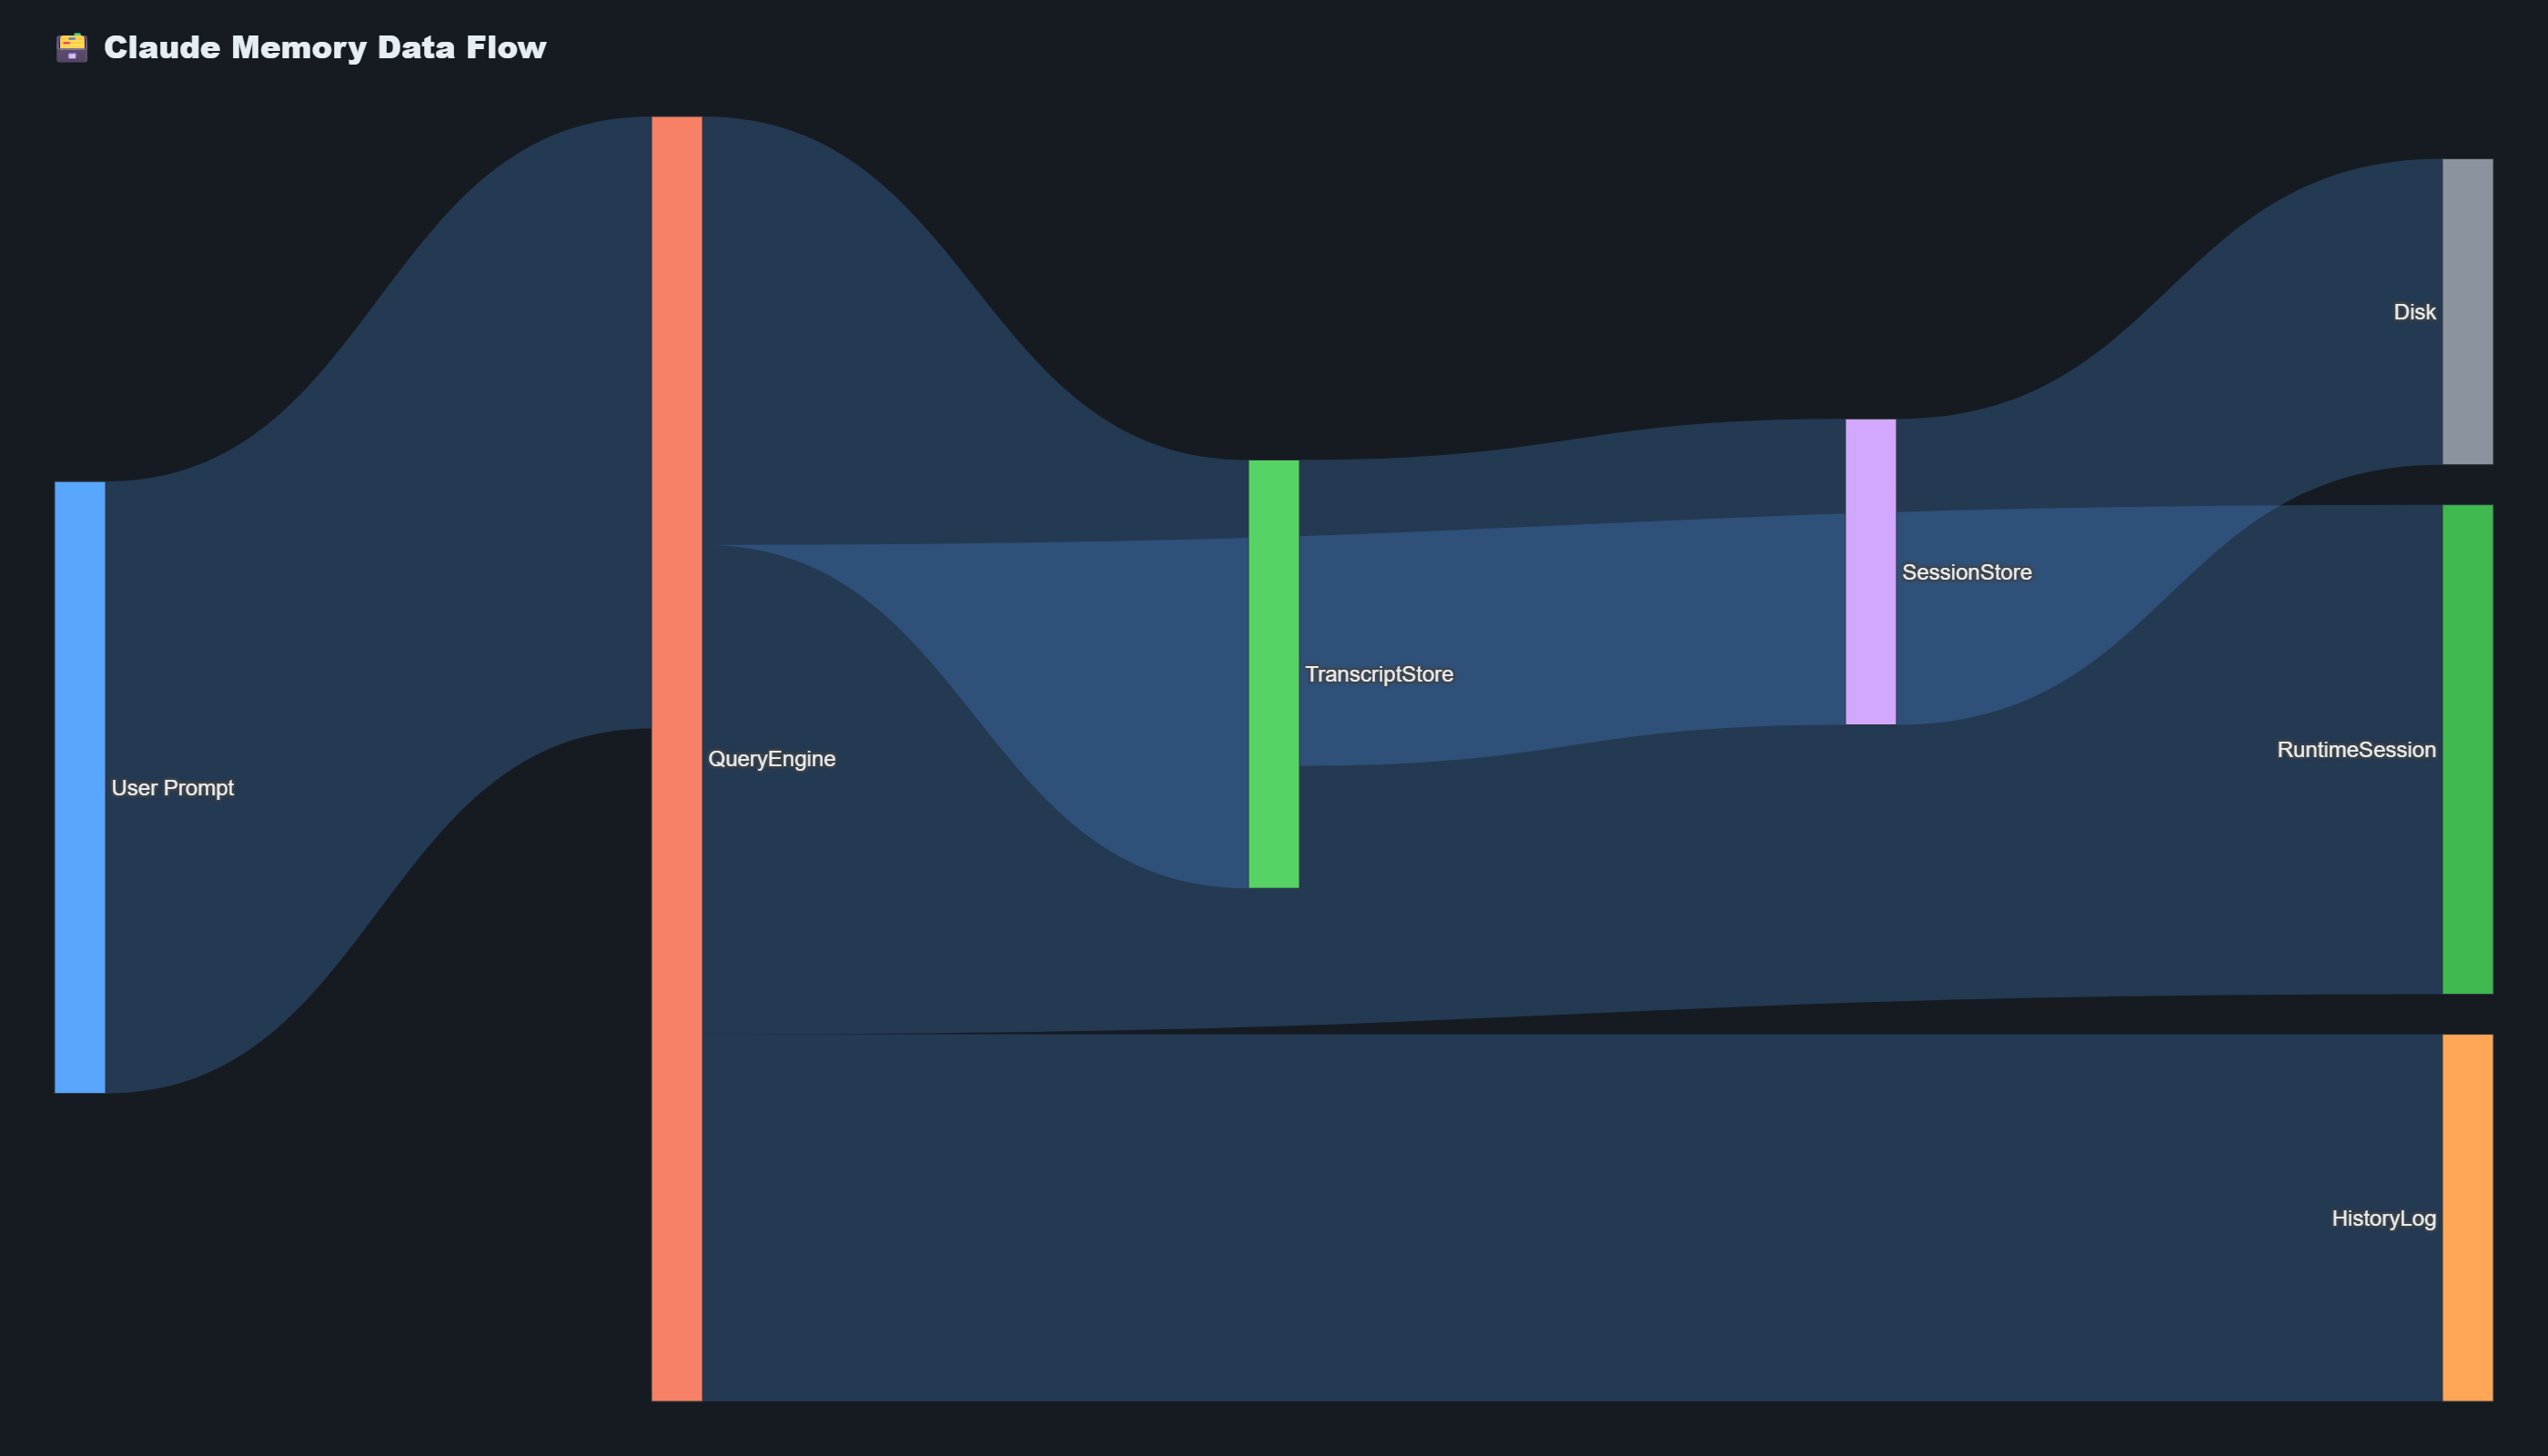
\includegraphics[width=\columnwidth]{05_memory_flow.png}
  \caption{Memory flow Sankey diagram. Data flows from the in-memory
    transcript (with \texttt{compact()} eviction) through
    \texttt{session\_store} to disk under \texttt{.port\_sessions/}.}
  \label{fig:mem_flow}
\end{figure}

\begin{lstlisting}[language=Python,
  caption={Memory eviction mechanism in \texttt{transcript.py}},
  label={lst:compact}]
def compact(self, keep_last: int = 10) -> None:
    """Truncate old turns to manage memory footprint."""
    if len(self._turns) > keep_last:
        self._turns = self._turns[-keep_last:]
\end{lstlisting}

\subsection{7-Stage Bootstrap Pipeline}

Every Claude Code invocation executes a fixed 7-stage initialization
sequence before processing any user request. This pipeline is
\emph{non-negotiable}: failure at any stage aborts the entire process
(Algorithm~\ref{alg:bootstrap}).

\begin{algorithm}[!t]
  \caption{Claude Code Bootstrap Pipeline}
  \label{alg:bootstrap}
  \begin{algorithmic}[1]
    \STATE \textbf{Stage 1:} Load configuration
    \STATE \textbf{Stage 2:} Initialize runtime environment
    \STATE \textbf{Stage 3:} Resolve module dependencies
    \STATE \textbf{Stage 4:} Setup system state
    \STATE \textbf{Stage 5:} Prefetch resources
    \STATE \textbf{Stage 6:} Establish query engine
    \STATE \textbf{Stage 7:} Prepare execution context
    \IF{any stage fails}
      \STATE Abort entire pipeline $\to$ fatal error
    \ENDIF
  \end{algorithmic}
\end{algorithm}

\begin{figure}[!t]
  \centering
  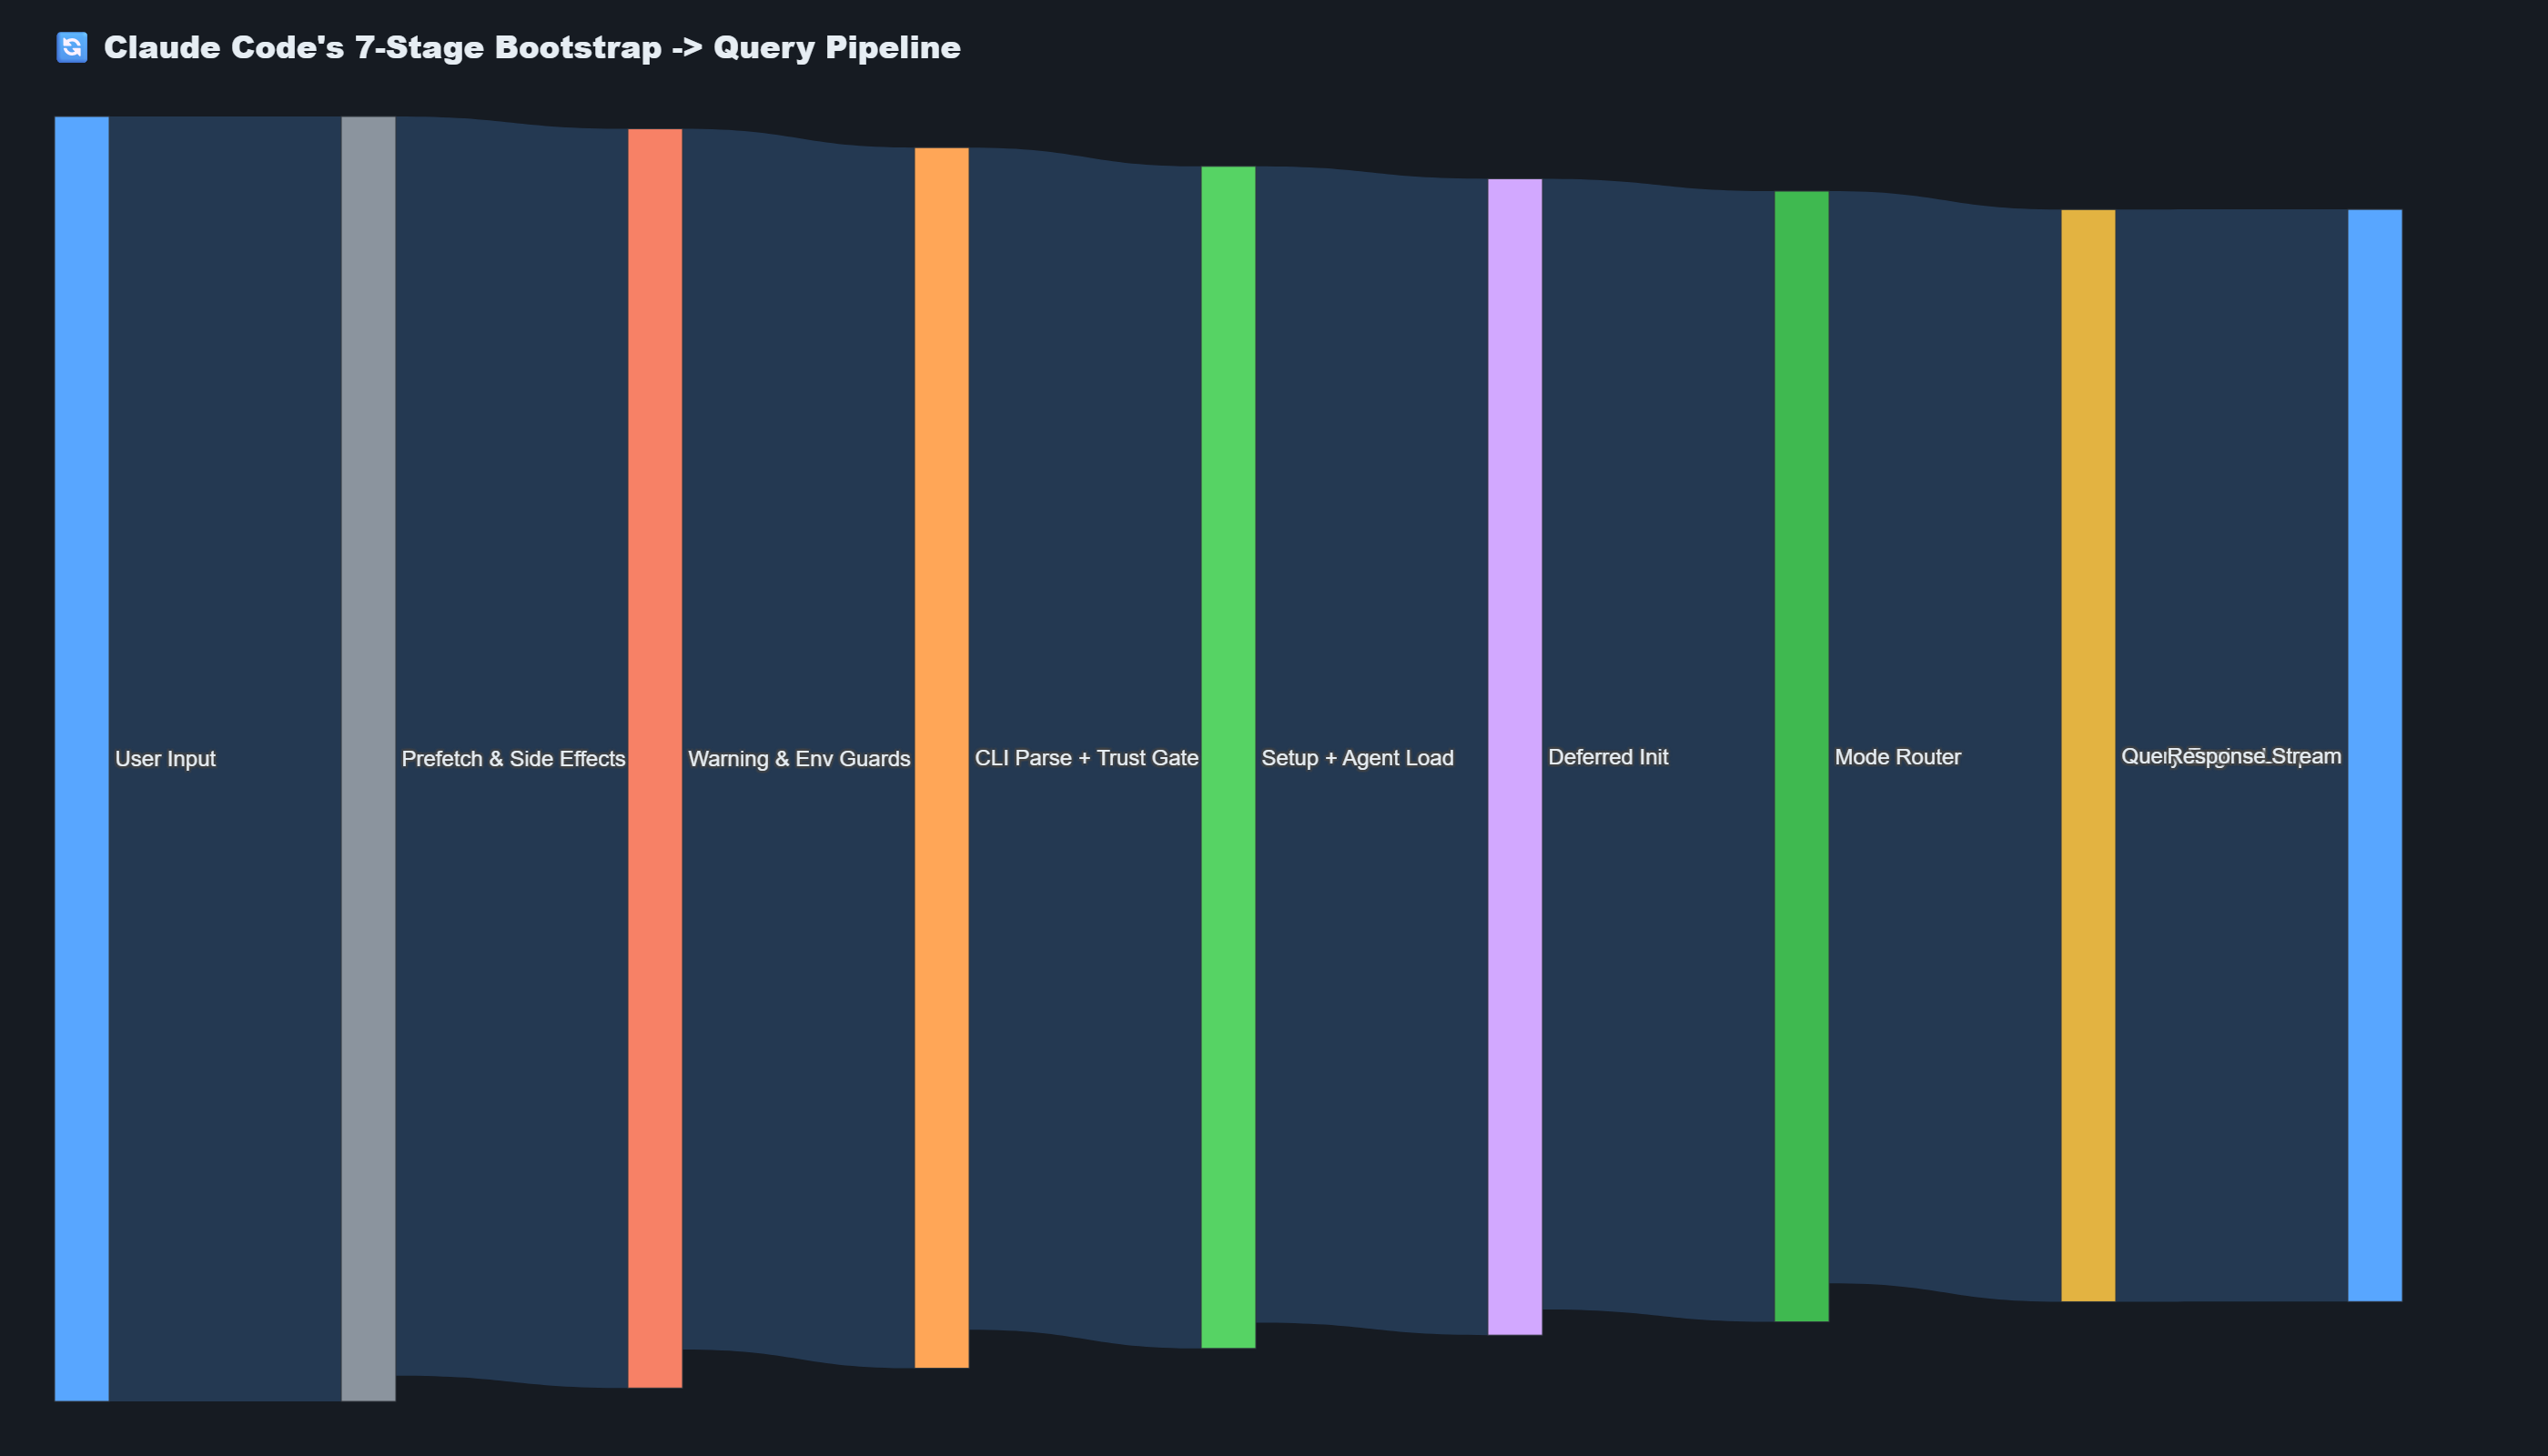
\includegraphics[width=\columnwidth]{08_bootstrap_pipeline.png}
  \caption{7-stage bootstrap pipeline visualized as a Sankey flow.
    Each stage is a mandatory gate; failure at any point prevents
    the agent from accepting user input.}
  \label{fig:pipeline}
\end{figure}

\subsection{Longest Dependency Chain}

After removing cycles and computing the DAG longest path, the deepest
transitive dependency chain spans 5 files:

\begin{equation}
  \small\texttt{main} \!\to\! \texttt{runtime} \!\to\! \texttt{sys\_init}
  \!\to\! \texttt{setup} \!\to\! \texttt{deferred\_init}
  \label{eq:chain}
\end{equation}

This moderate depth indicates deliberate separation of concerns,
avoiding the deep coupling seen in poorly structured codebases.
Figure~\ref{fig:chain} highlights this chain within the full
import network.

\begin{figure}[!t]
  \centering
  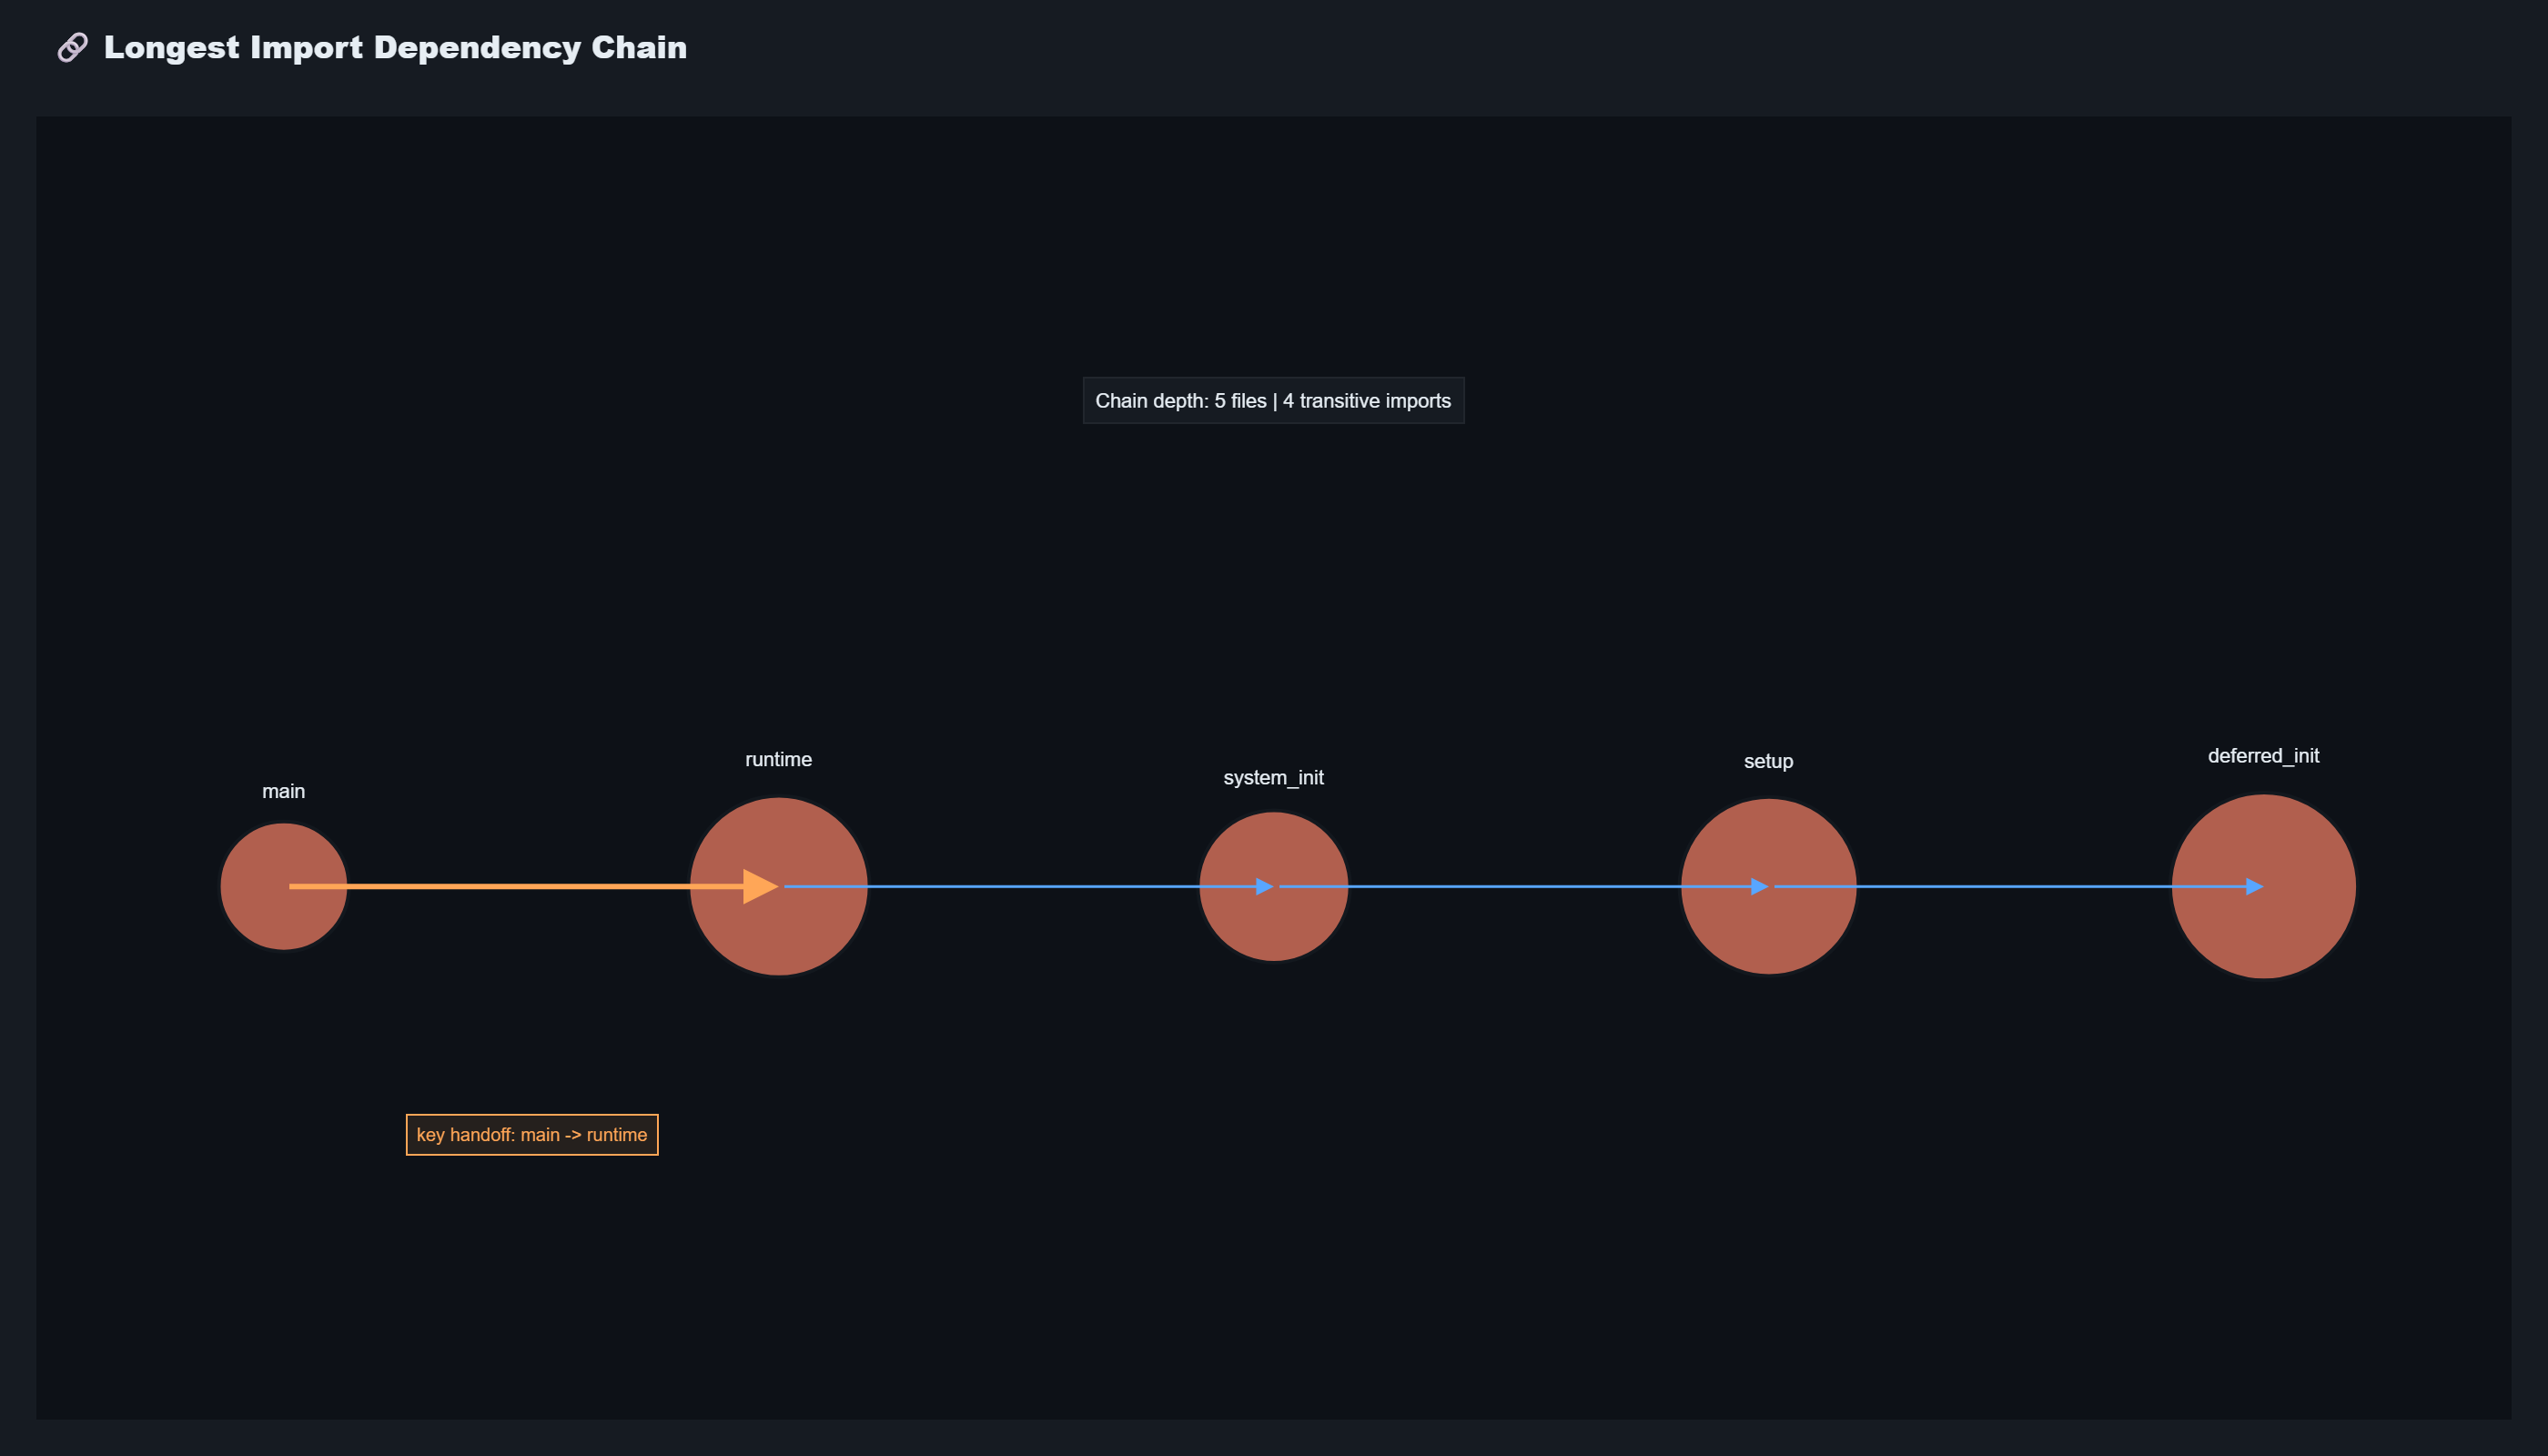
\includegraphics[width=\columnwidth]{09_dependency_chain.png}
  \caption{Longest transitive dependency chain (5 files) highlighted
    in the import graph. Node size encodes PageRank; the chain
    \texttt{main}$\to\cdots\to$\texttt{deferred\_init} is traced
    in a contrasting color.}
  \label{fig:chain}
\end{figure}

\subsection{Subsystem Composition}

Table~\ref{tab:subsystems} shows the module distribution across the
15 largest of the 29 total subsystems. The \texttt{utils} subsystem
(564 modules, 29.6\%) and \texttt{components} (389 modules, 20.4\%)
together account for half the entire codebase, reflecting significant
investment in foundational infrastructure.

\begin{table}[!t]
  \renewcommand{\arraystretch}{1.25}
  \caption{Top 15 Subsystems by Module Count}
  \label{tab:subsystems}
  \centering
  \begin{tabular}{@{}lrl@{}}
    \toprule
    \textbf{Subsystem} & \textbf{Modules} & \textbf{Share} \\
    \midrule
    utils       & 564 & 29.6\% \\
    components  & 389 & 20.4\% \\
    services    & 130 &  6.8\% \\
    hooks       & 104 &  5.5\% \\
    bridge      &  31 &  1.6\% \\
    constants   &  21 &  1.1\% \\
    skills      &  20 &  1.1\% \\
    cli         &  19 &  1.0\% \\
    keybindings &  14 &  0.7\% \\
    types       &  11 &  0.6\% \\
    migrations  &  11 &  0.6\% \\
    memdir      &   8 &  0.4\% \\
    entrypoints &   8 &  0.4\% \\
    state       &   6 &  0.3\% \\
    buddy       &   6 &  0.3\% \\
    \bottomrule
  \end{tabular}
\end{table}

\subsection{Feature Flags}

The feature-flag scan identified only \textbf{4 boolean flags} across
all 66 modules, listed in Table~\ref{tab:flags}. This sparsity
suggests the development team deliberately ships behavior as
deterministic logic rather than configurable toggles, prioritizing
predictability over runtime flexibility.

\begin{table}[!t]
  \renewcommand{\arraystretch}{1.25}
  \caption{Feature Flags Detected Across All 66 Modules}
  \label{tab:flags}
  \centering
  \begin{tabular}{@{}llll@{}}
    \toprule
    \textbf{Module}         & \textbf{Flag}    & \textbf{Default}    & \textbf{State} \\
    \midrule
    \texttt{direct\_modes}  & \texttt{active}  & \texttt{True}       & On  \\
    \texttt{runtime}        & \texttt{trusted} & \texttt{True}       & On  \\
    ---                     & ---              & \texttt{False}      & Off \\
    ---                     & ---              & \texttt{False}      & Off \\
    \bottomrule
  \end{tabular}
\end{table}

\begin{figure}[!t]
  \centering
  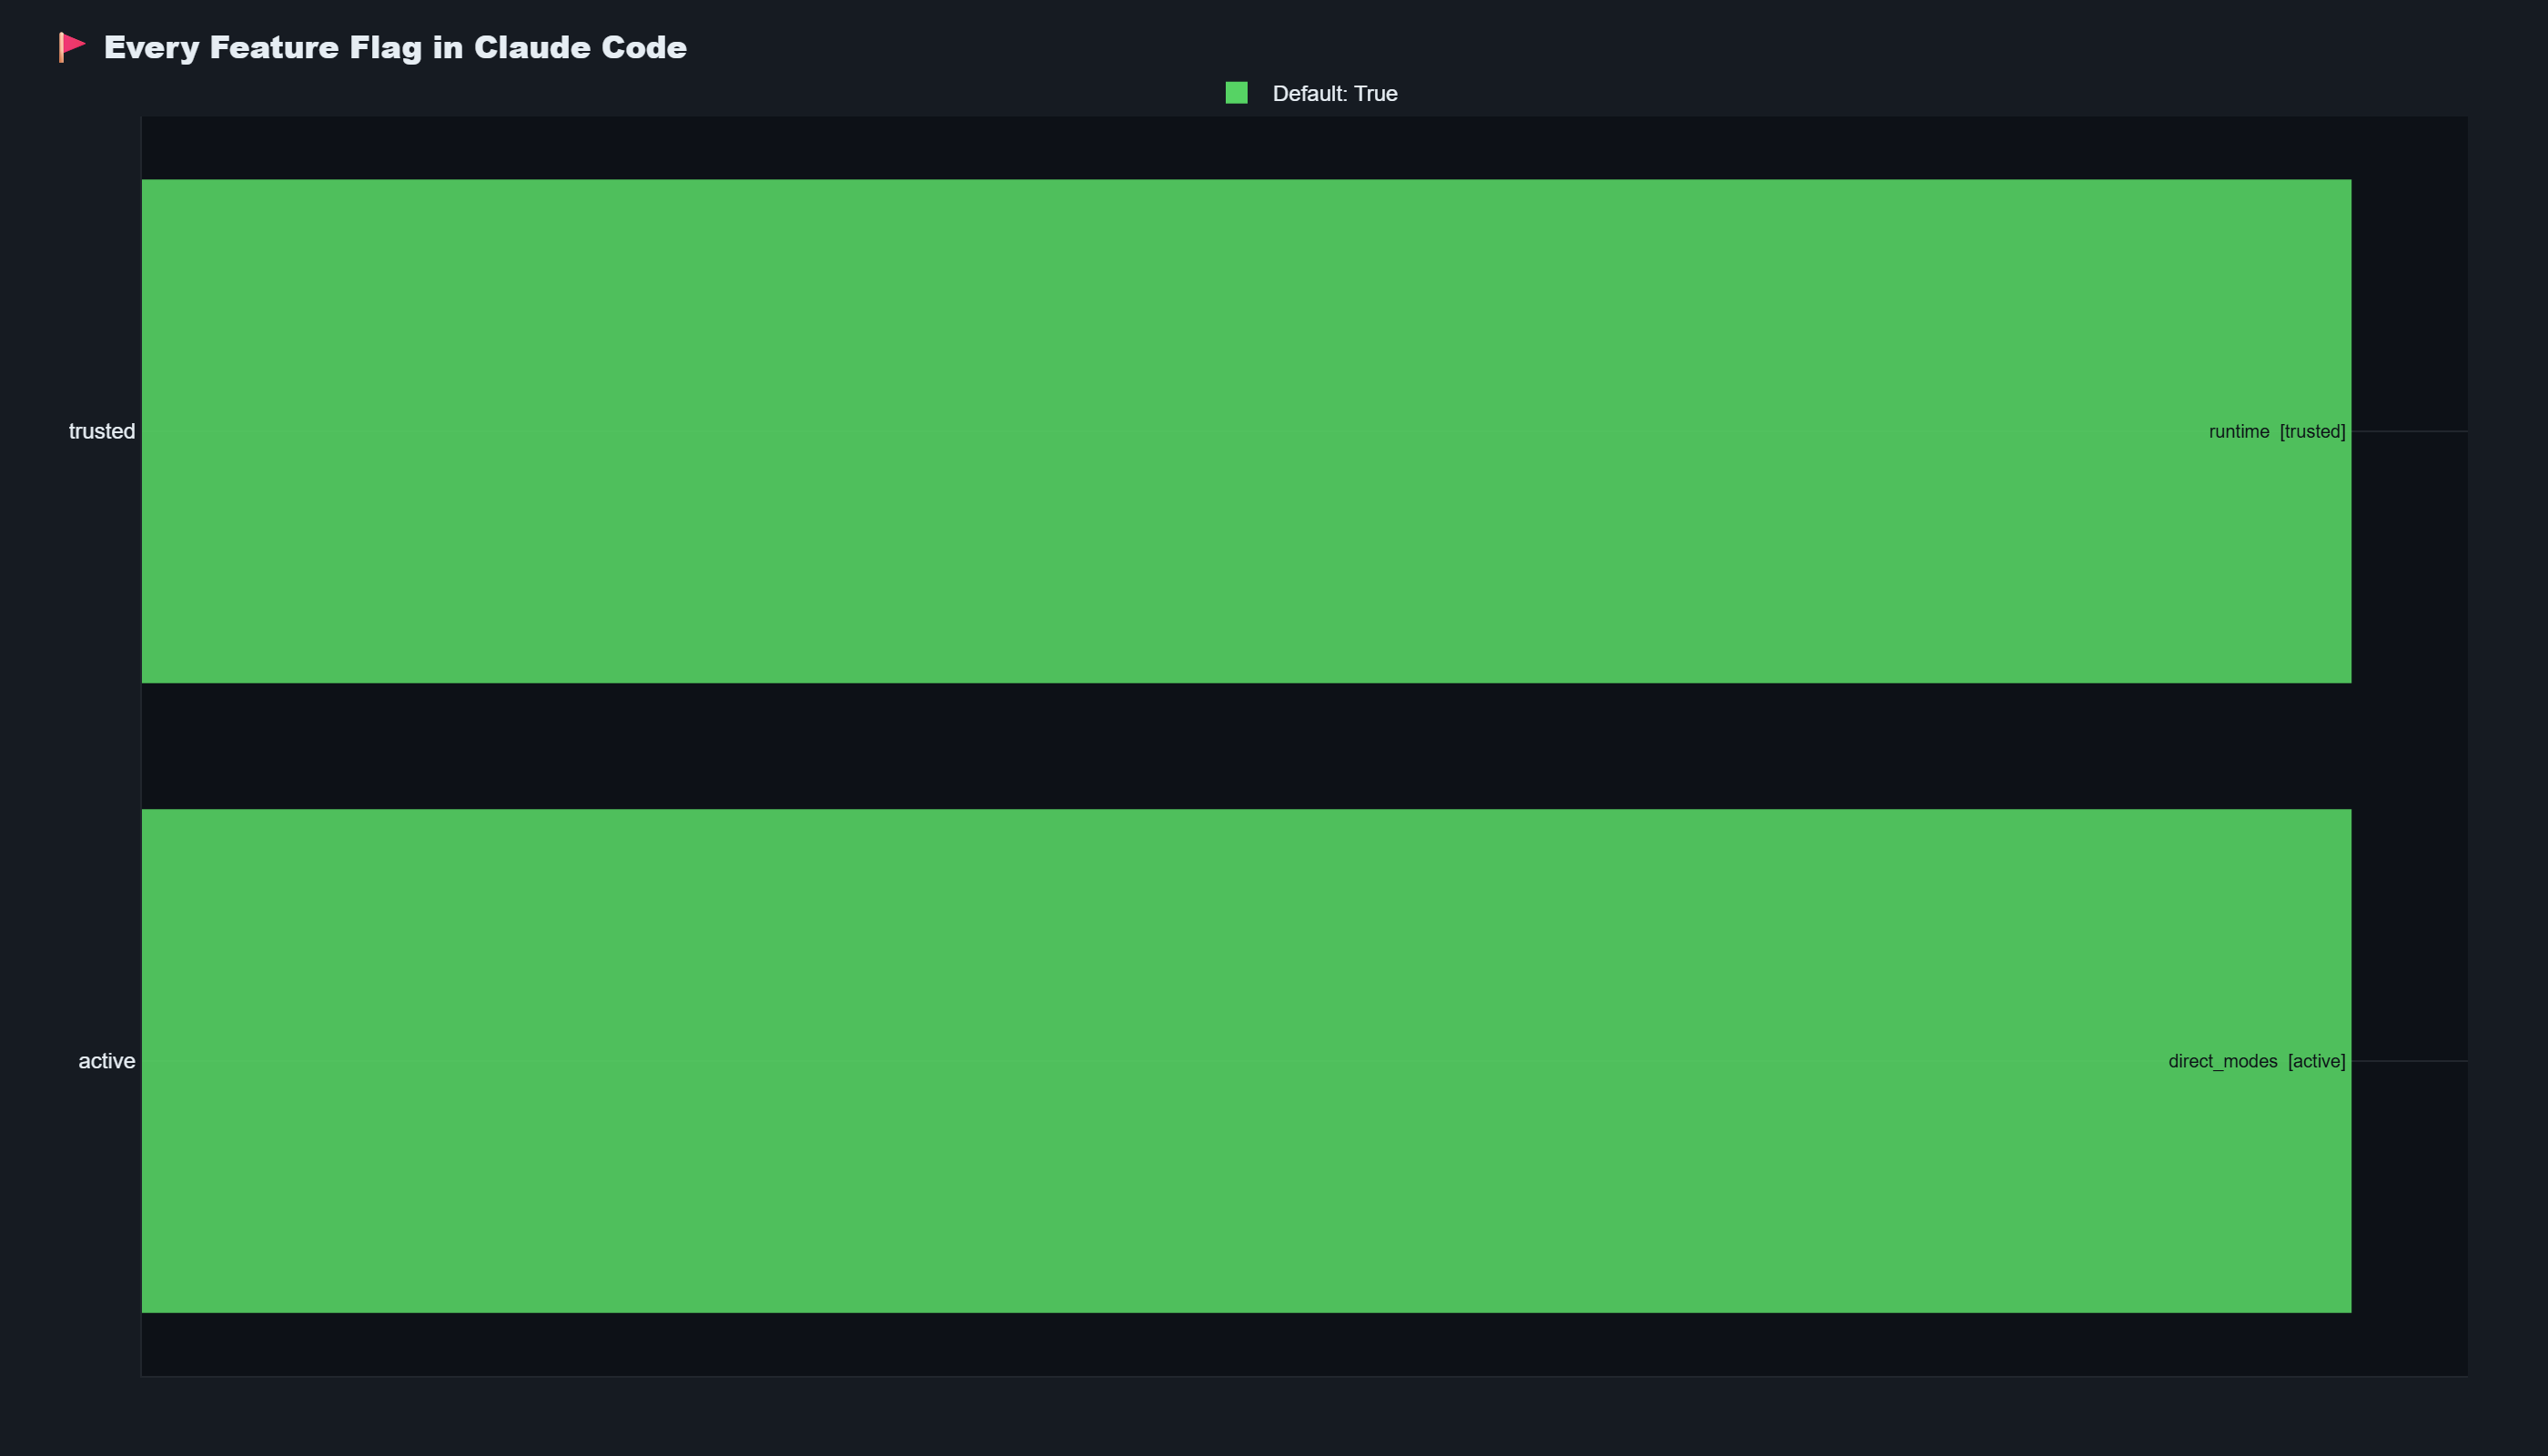
\includegraphics[width=\columnwidth]{07_feature_flags.png}
  \caption{All 4 detected feature flags. Green bars are \texttt{True}
    by default; red bars are \texttt{False}. Near-absence of flags
    across 66 modules reflects a deliberate architectural stance.}
  \label{fig:flags}
\end{figure}

\subsection{String Constants and Hardcoded Directives}

AST extraction identified \textbf{64 string constants $\geq 40$
characters} embedded in the source. The five longest are:

\begin{enumerate}
  \item (88 chars, \texttt{main}): \textit{``compare the Python workspace
    against the local ignored TypeScript archive...''}
  \item (86 chars, \texttt{replLauncher}): \textit{``Python porting REPL is
    not interactive yet; use \texttt{python3 -m src.main summary}...''}
  \item (85 chars, \texttt{parity\_audit}): \textit{``Local archive
    unavailable; parity audit cannot compare against the
    original snapshot.''}
  \item (74 chars, \texttt{bootstrap\_graph}): \textit{``mode routing:
    local / remote / ssh / teleport / direct-connect / deep-link''}
\end{enumerate}

These strings reveal internal routing labels, operational mode
identifiers, and developer-facing diagnostics embedded directly in
the compiled source. Figure~\ref{fig:topics} groups all 64 strings
by inferred topic cluster.

\begin{figure}[!t]
  \centering
  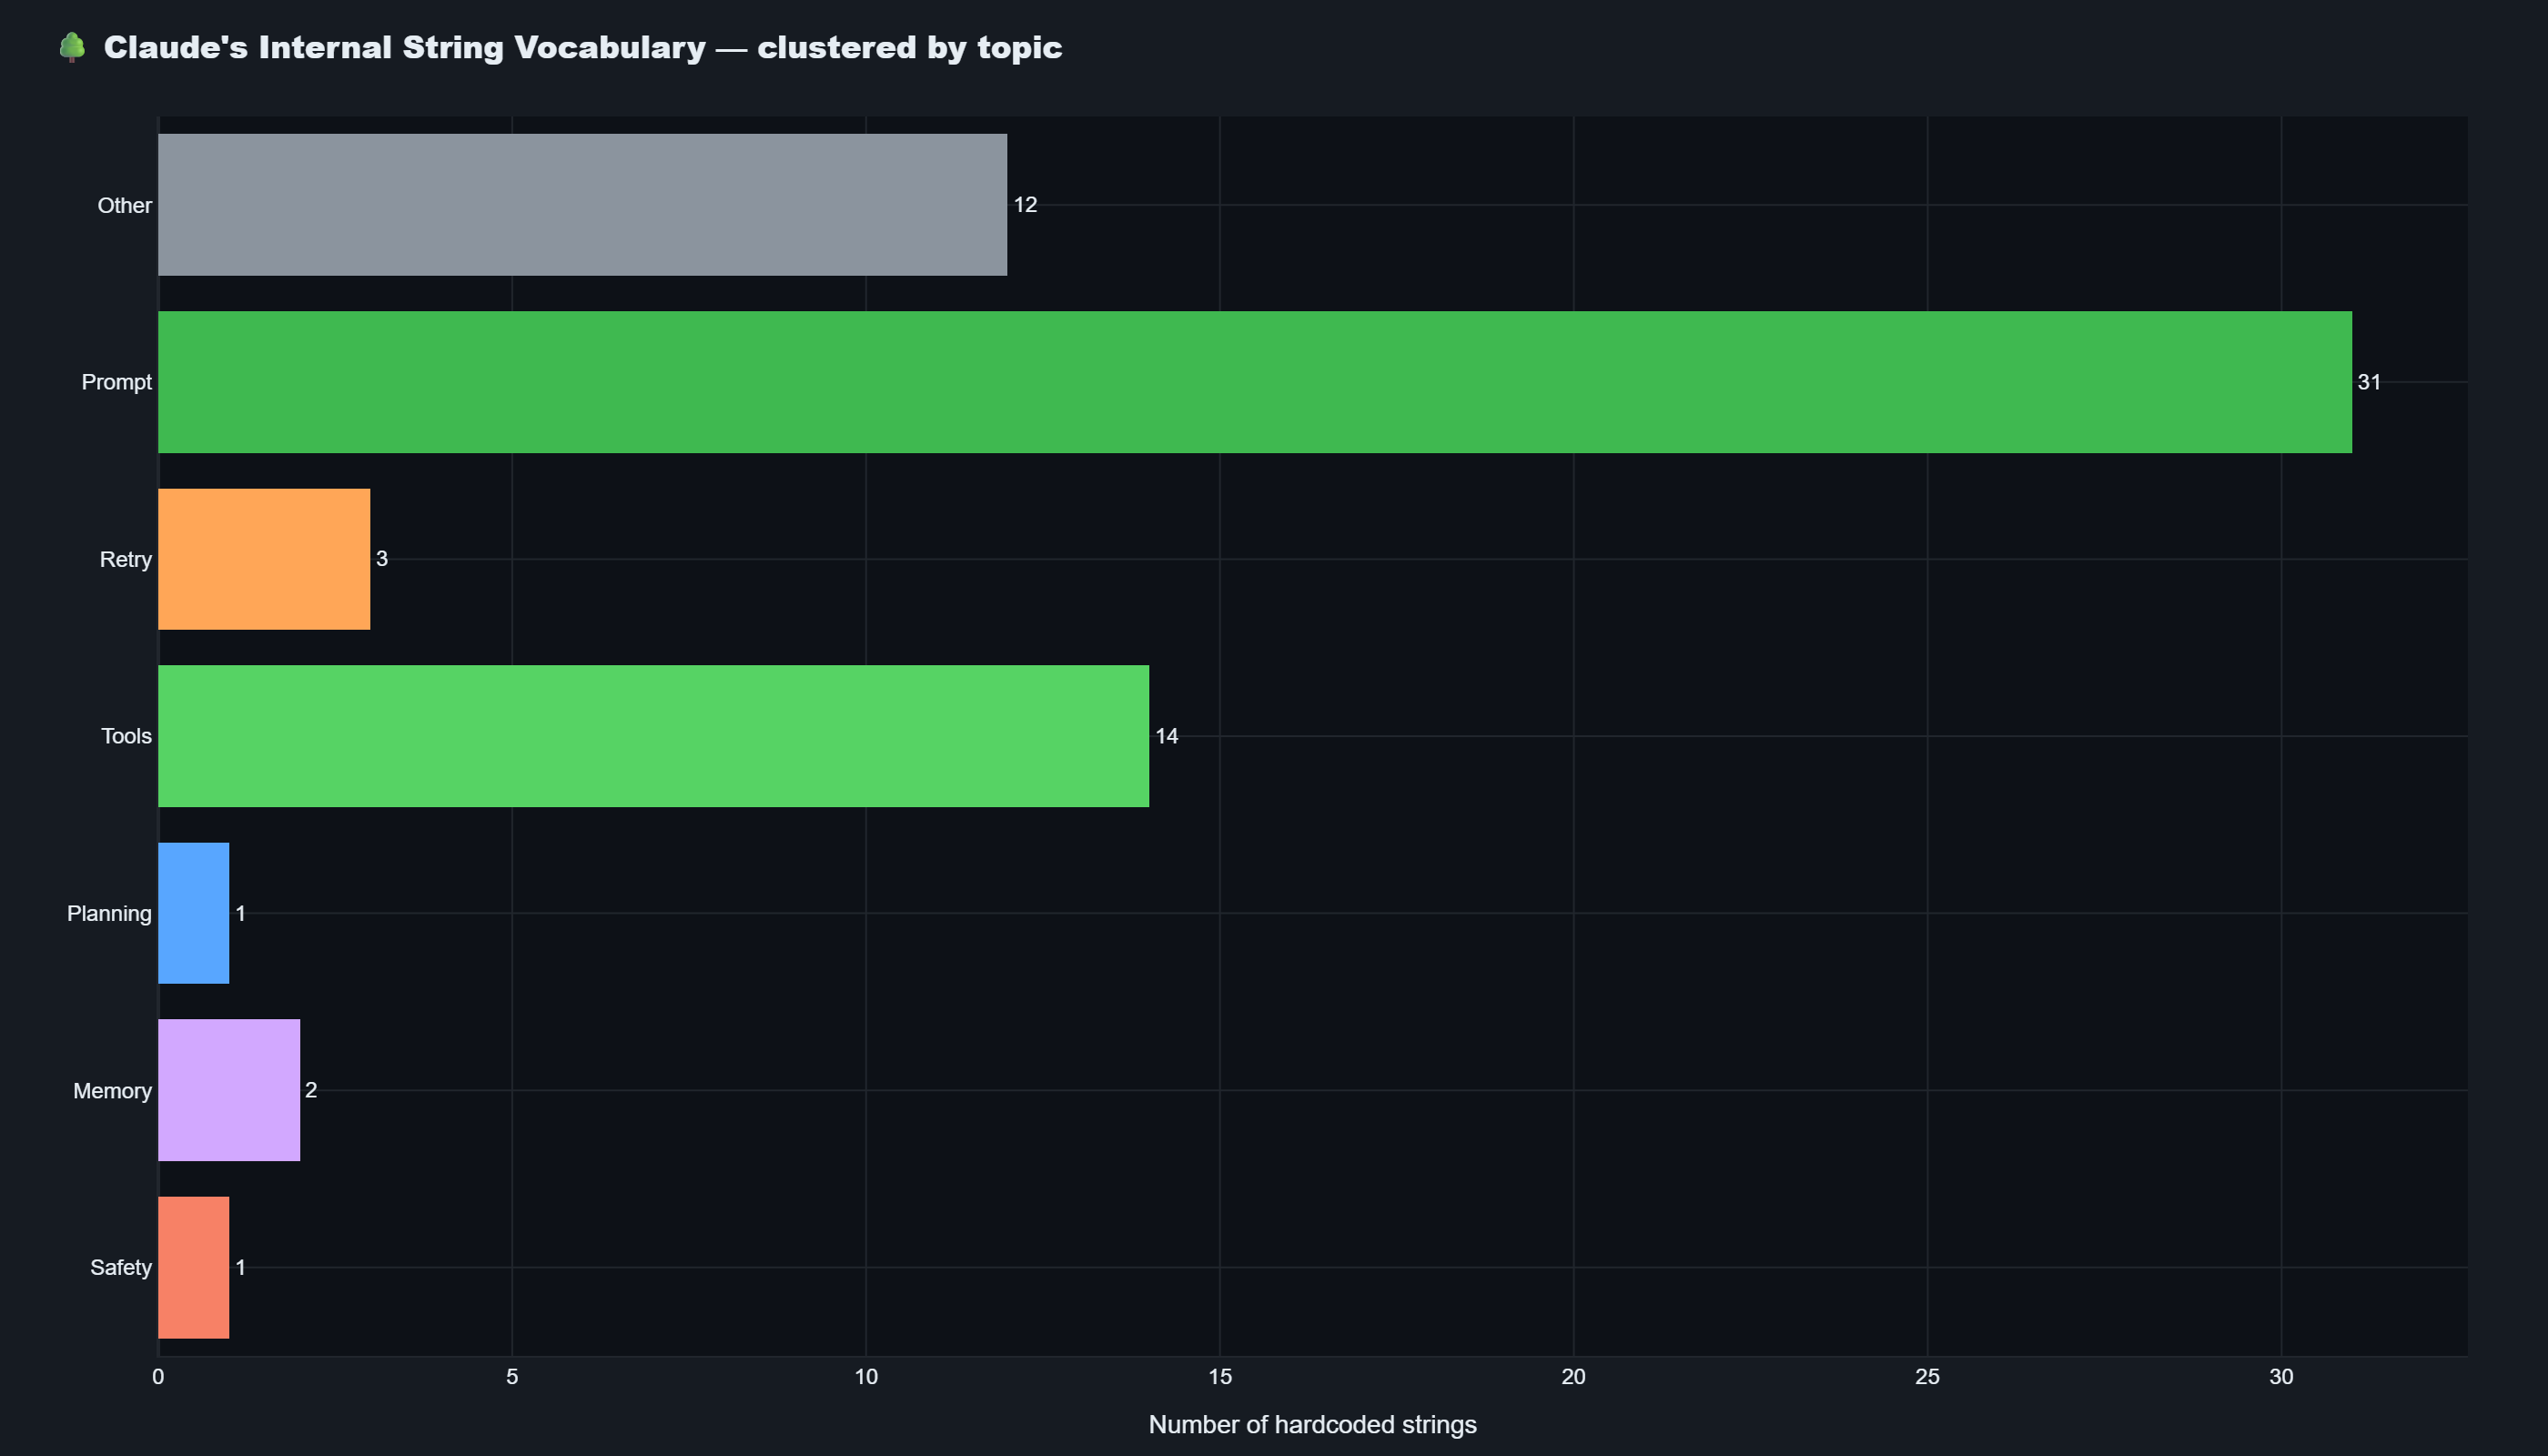
\includegraphics[width=\columnwidth]{04_string_topics.png}
  \caption{Hardcoded string constants ($\geq$40 chars) extracted via
    AST analysis, grouped by topic cluster, revealing the internal
    vocabulary of Claude Code's behavioral directives.}
  \label{fig:topics}
\end{figure}

Figure~\ref{fig:ct} shows the distribution of slash commands and
registered tools across subsystems.

\begin{figure}[!t]
  \centering
  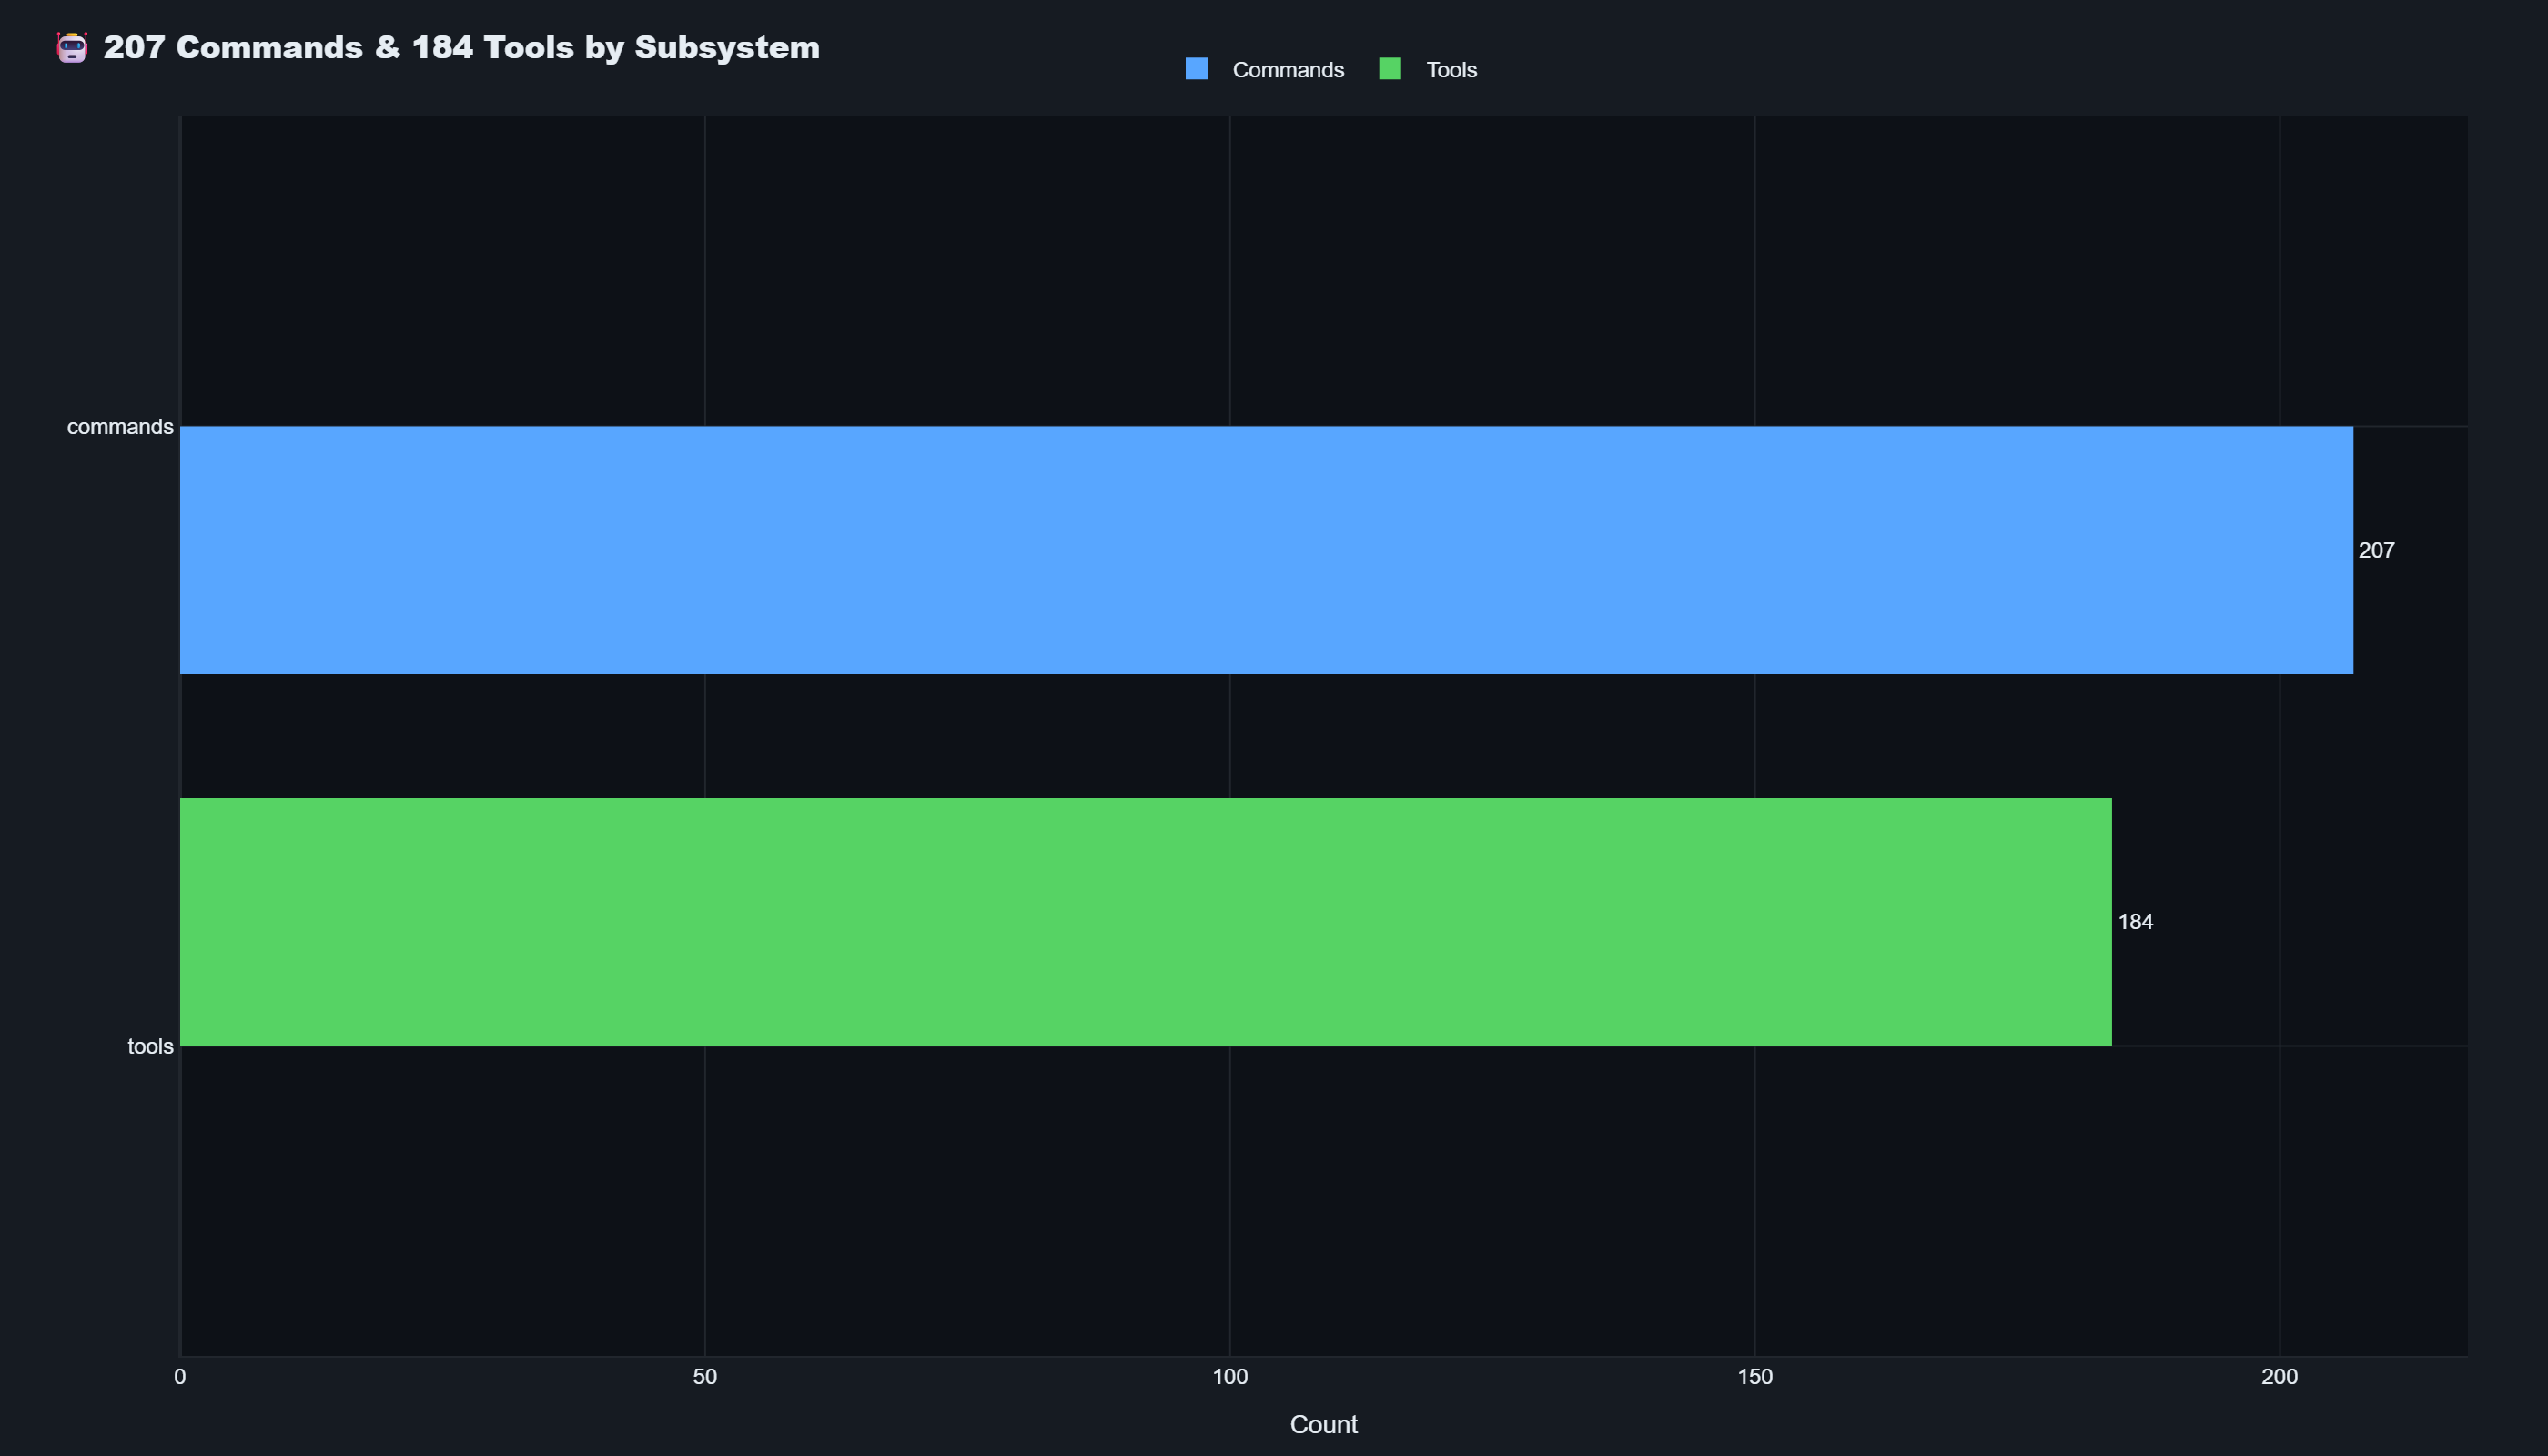
\includegraphics[width=\columnwidth]{06_commands_tools.png}
  \caption{207 slash commands and 184 registered tools distributed
    across subsystems. Disparity in density reveals which areas own
    the most user-facing functionality.}
  \label{fig:ct}
\end{figure}

% Wide figures --- placed at top of their respective pages
\begin{figure*}[!t]
  \centering
  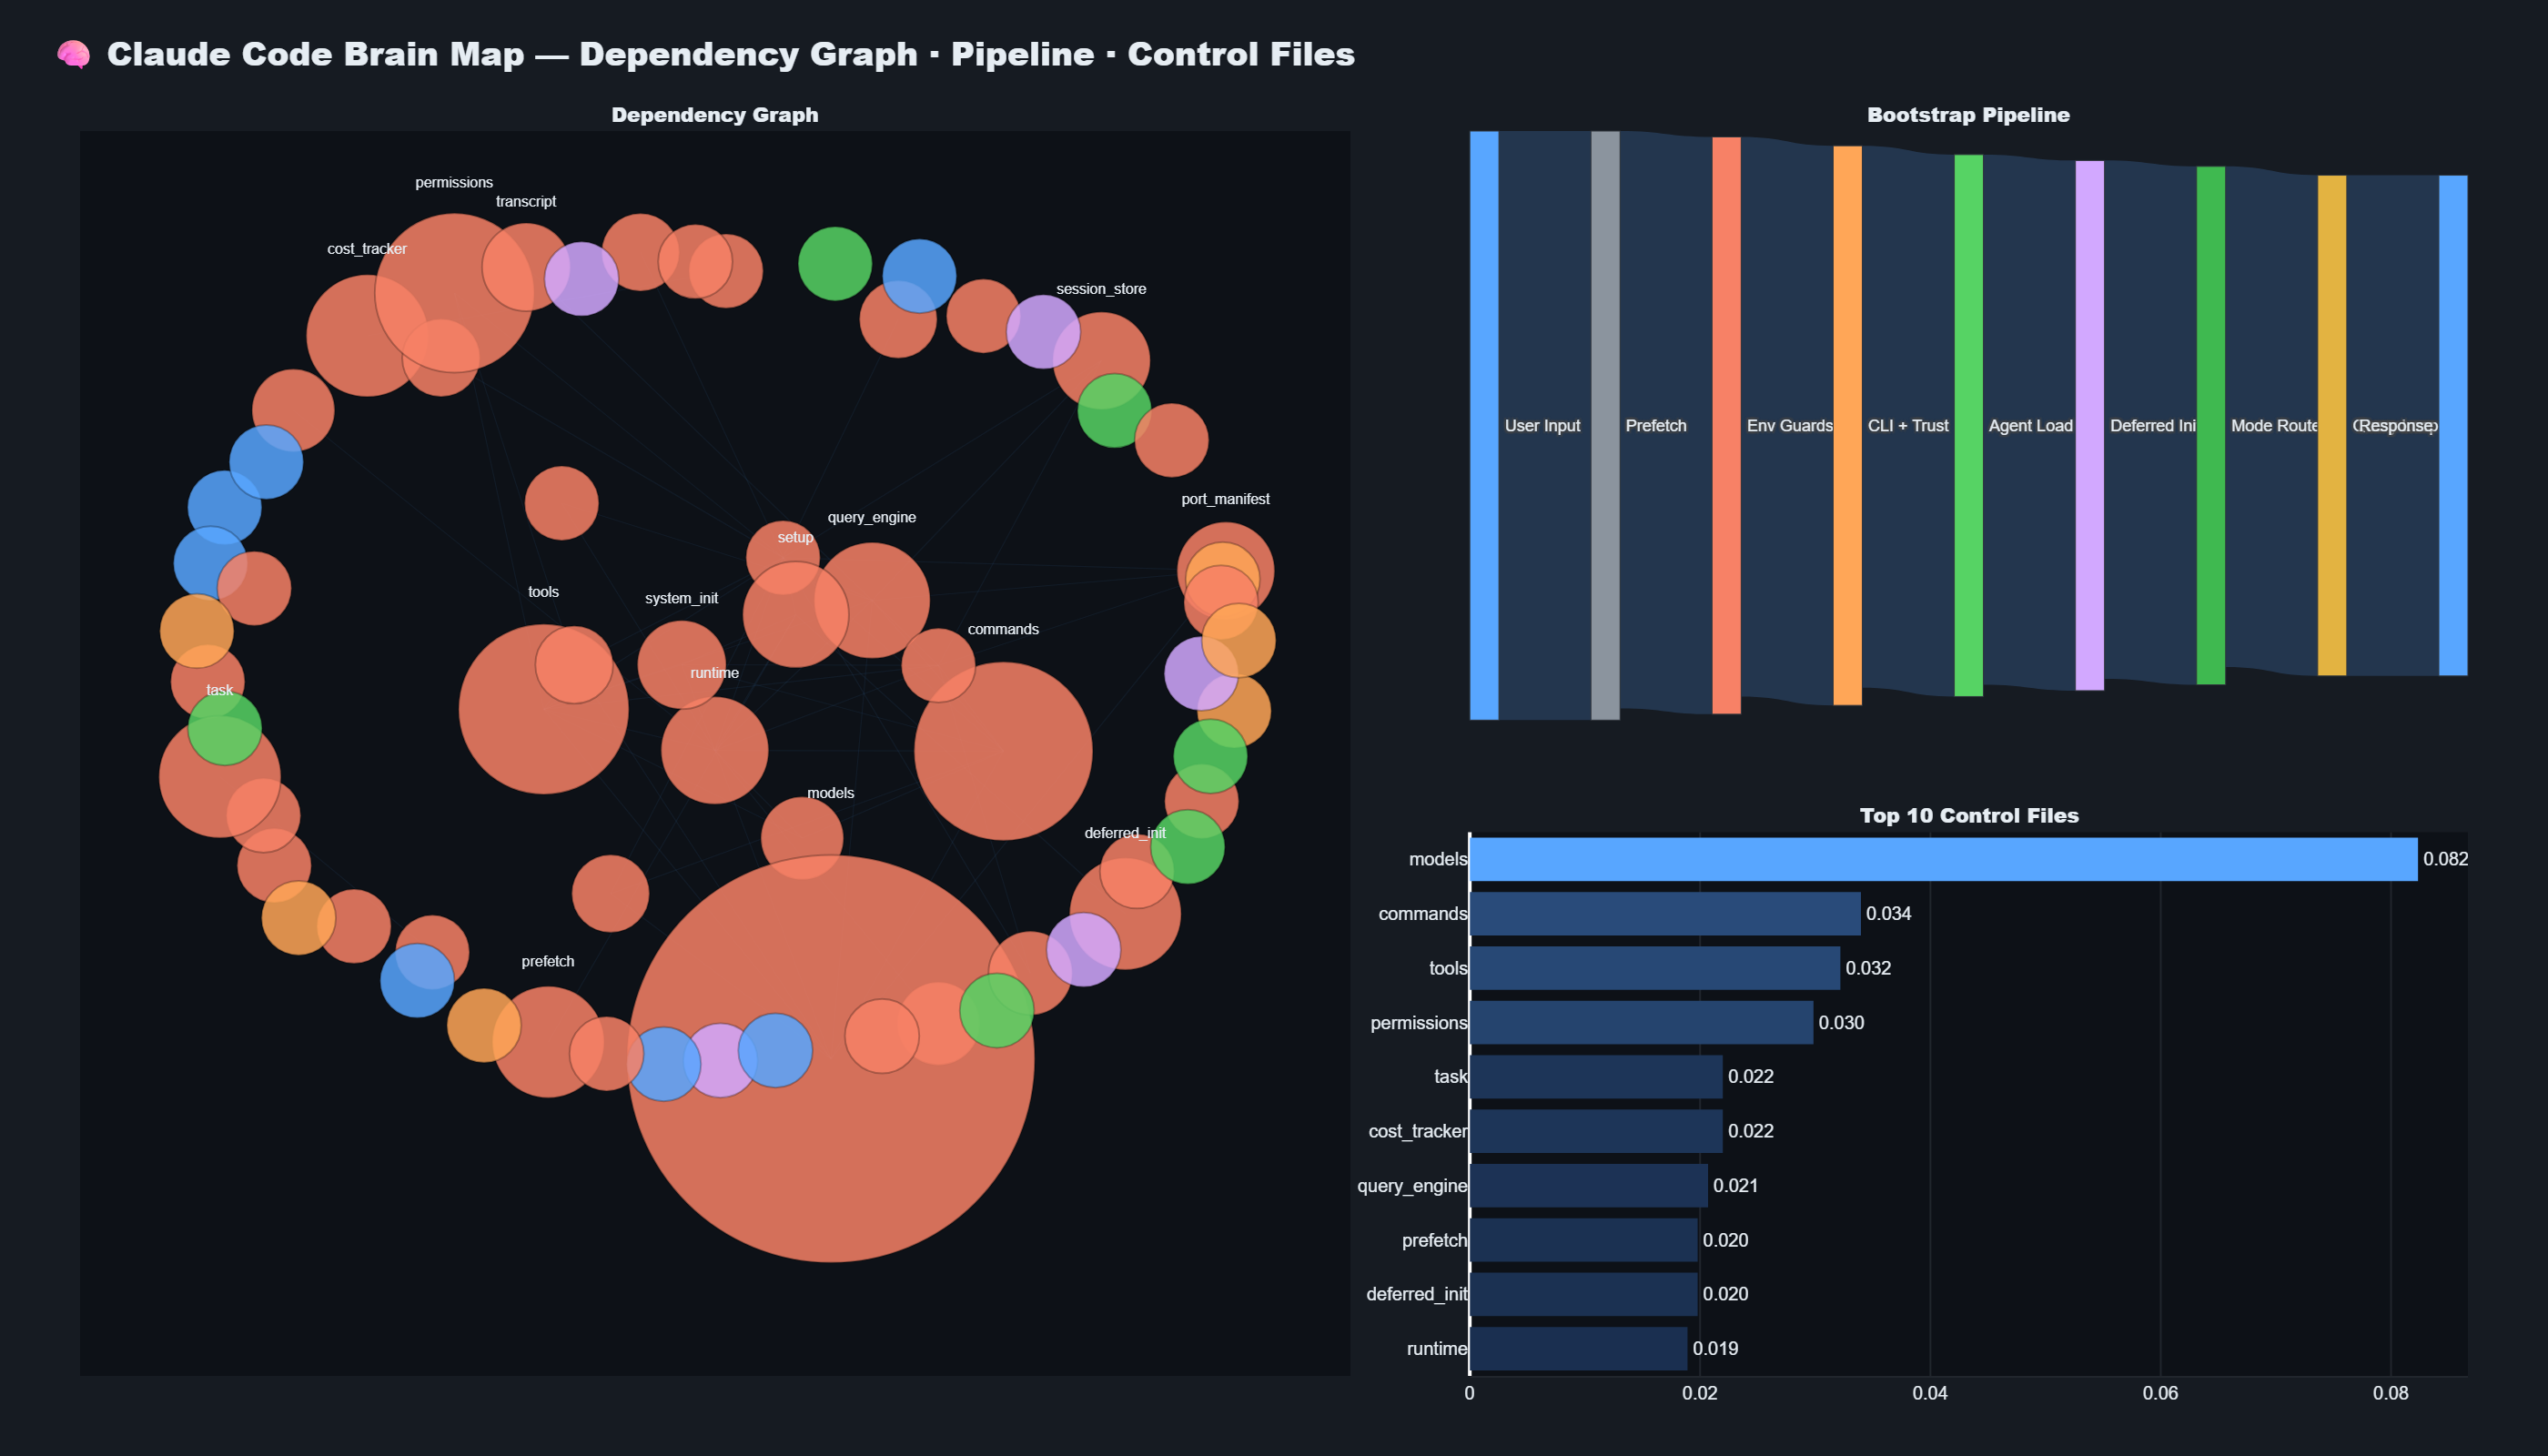
\includegraphics[width=\textwidth]{02_hero_overview.png}
  \caption{Hero composite: (\textit{left})~dependency graph,
    (\textit{top-right})~7-stage bootstrap pipeline flow,
    (\textit{bottom-right})~top-10 critical files by PageRank.
    Together these three panels capture the full structural picture
    of Claude Code.}
  \label{fig:hero}
\end{figure*}

\begin{figure*}[!t]
  \centering
  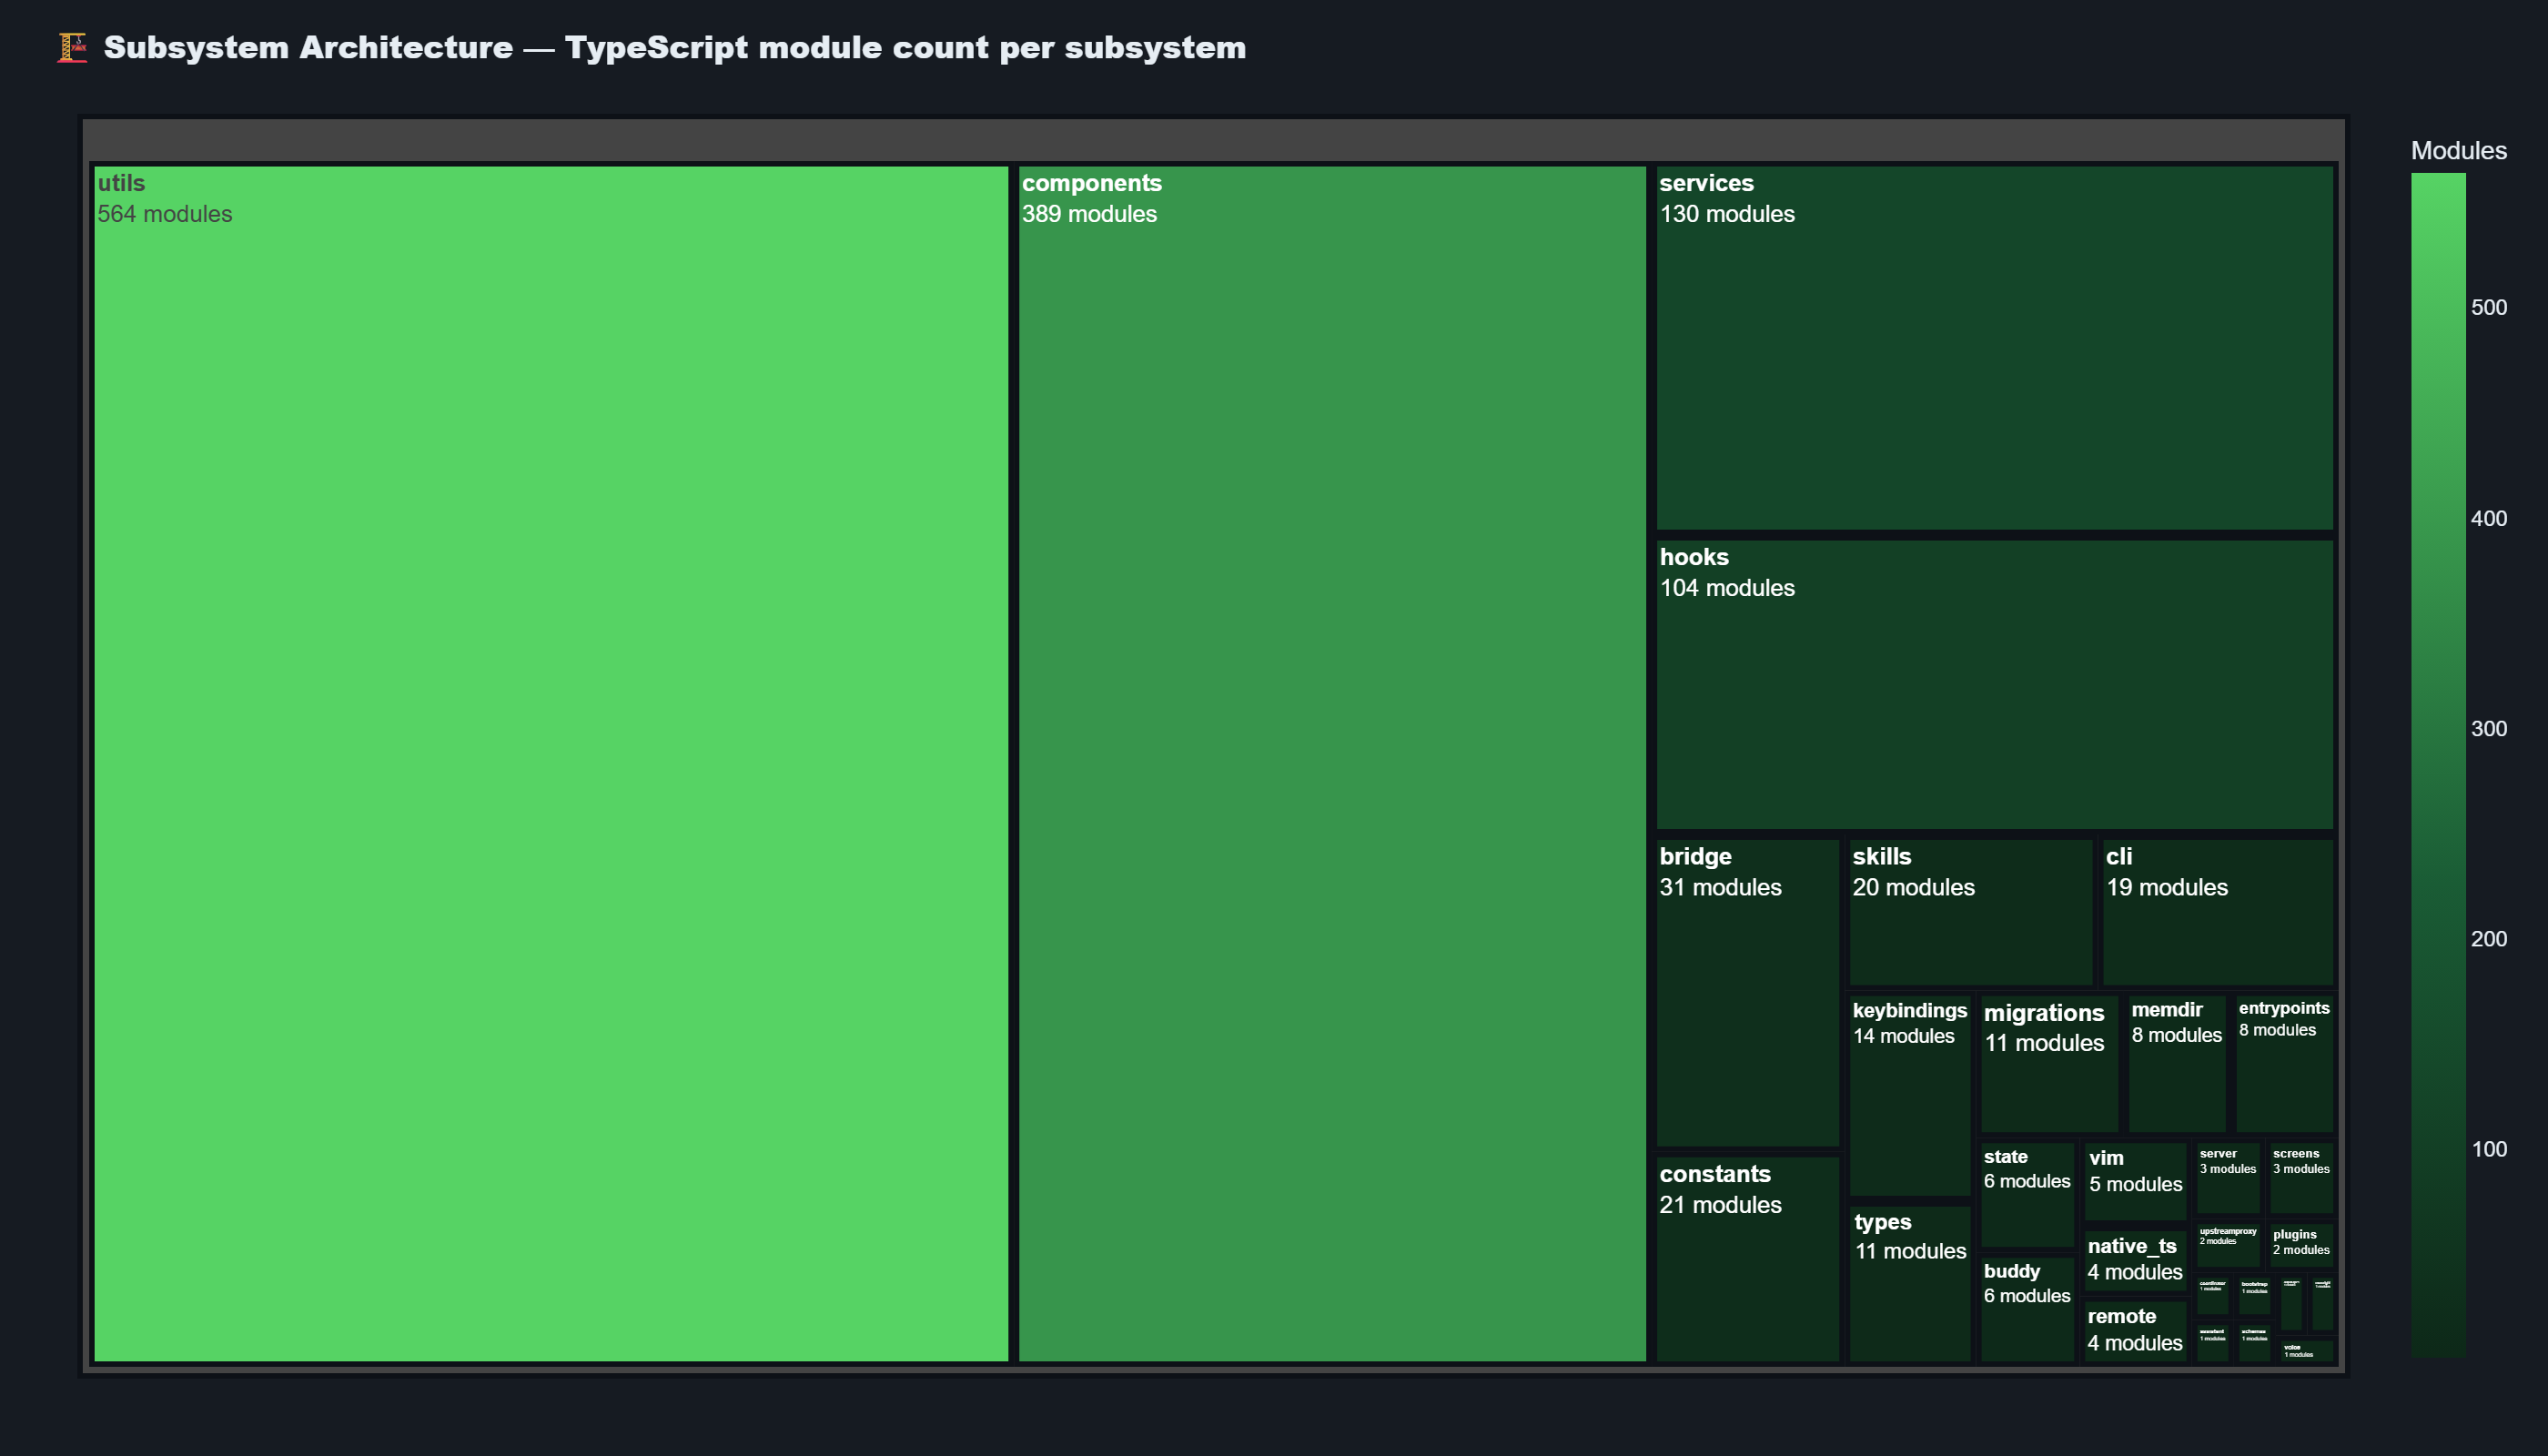
\includegraphics[width=\textwidth]{11_subsystem_architecture.png}
  \caption{Subsystem architecture treemap across all 29 subsystems.
    Area $\propto$ module count. \texttt{utils} (564) and
    \texttt{components} (389) together represent 50\% of the original
    TypeScript codebase.}
  \label{fig:treemap}
\end{figure*}

% ---------------------------------------------------------------
\section{Discussion}
% ---------------------------------------------------------------

\subsection{Architectural Brittleness at the Core}

The 15\% import concentration through
$\texttt{models} \to \texttt{commands} \to \texttt{tools}$ represents
a classical \emph{God Object} anti-pattern~\cite{brown1998antipatterns}
at the module level. While this centralization simplifies routing
logic, it creates a fragile axis: any breaking change to
\texttt{models} propagates immediately to both \texttt{commands} and
\texttt{tools}, affecting the entirety of the command and tool
dispatch surfaces.

From an evolutionary architecture
perspective~\cite{ford2017evolutionary}, decoupling this axis would
be the highest-leverage refactoring opportunity in the codebase.

\subsection{Memory as a Finite Resource}

The \texttt{compact(keep\_last=10)} mechanism represents a deliberate
\emph{finite memory contract}. Rather than relying on the LLM's native
context window, the system enforces its own eviction policy at the
application layer:

\begin{enumerate}
  \item Claude's apparent forgetfulness in long sessions is a software
        policy, not a model capability limitation.
  \item The threshold (10 turns) can theoretically be tuned.
  \item Session persistence via \texttt{session\_store.py} coexists
        with in-memory eviction, suggesting sessions are recoverable
        after compaction via disk lookup.
\end{enumerate}

\subsection{Bootstrap Pipeline Robustness}

The 7-stage sequential pipeline is a fail-fast design: any stage
failure aborts immediately. While this simplifies error propagation,
it means configuration errors (Stage 1) and dependency resolution
failures (Stage 3) produce the same user-facing symptom: a
non-starting agent. Improved error messages distinguishing pipeline
stage failures would significantly aid diagnostics.

\subsection{Feature Flag Minimalism}

With only 4 feature flags, Claude Code occupies the minimal end of
the \emph{configurability spectrum}~\cite{neri2013software}. LLM
agents with many configurable toggles introduce combinatorial
behavior spaces that are difficult to test and reason about. Claude
Code instead hardcodes behavior, trading configurability for
predictability --- a defensible choice for a production AI tool.

\subsection{Utility Subsystem Dominance}

The \texttt{utils} (564 modules) and \texttt{components} (389
modules) subsystems account for 50\% of the TypeScript codebase.
This is consistent with mature systems where foundational
infrastructure outweighs feature code, and suggests Claude Code's
extensibility surface is primarily component-based rather than
service-based.

% ---------------------------------------------------------------
\section{Threats to Validity}
% ---------------------------------------------------------------

\subsection{Internal Validity}

The analysis targets \texttt{claw-code}, a Python \emph{port} of
Claude Code, not the original TypeScript source. Porting may have
introduced structural changes not present in the original
architecture. String stripping, comment removal, and import
reorganization could affect our findings.

\subsection{External Validity}

Our findings apply to the version of \texttt{claw-code} available
at analysis time (April 2026). Anthropic may have shipped
architectural changes in newer Claude Code versions. The
\texttt{compact()} threshold, pipeline stages, and feature flags
should be treated as version-specific findings.

\subsection{Construct Validity}

PageRank centrality measures \emph{import-graph influence}, a proxy
for architectural criticality but not a direct measure of runtime
importance. A module with high PageRank might be critical at load
time but rarely executed at runtime, and vice versa.

% ---------------------------------------------------------------
\section{Conclusion}
% ---------------------------------------------------------------

We presented \emph{Claude X-Ray}, a static analysis study of the
internal architecture of Claude Code via its open Python port
\texttt{claw-code}. Our analysis reveals:

\begin{itemize}
  \item A 15\% import bottleneck through
        \texttt{models $\to$ commands $\to$ tools} creating a systemic
        fragility axis.
  \item An explicit memory eviction policy (\texttt{compact(keep\_last=10)})
        that explains Claude's observed long-session behavior.
  \item A strict 7-stage bootstrap pipeline where any initialization
        failure is catastrophic.
  \item A minimal feature-flag surface (4 flags) reflecting a deliberate
        design philosophy of predictability over configurability.
  \item \texttt{query\_engine} as the highest-PageRank node and de facto
        architectural center of the system.
\end{itemize}

These findings are actionable: developers extending Claude Code should
treat the \texttt{models/commands/tools} axis as a fragile zone; users
experiencing long-session degradation should understand it as an
intentional policy; researchers studying LLM agent design can use
Claude Code as a case study in minimalist, deterministic agent
architecture.

Future work includes dynamic analysis (runtime profiling of the
bootstrap pipeline), comparative analysis against LangChain and
AutoGen, and architectural evolution tracking as Claude Code versions
are released.

% ---------------------------------------------------------------
\appendix
\section{Reproducibility}

All analyses were performed in a Jupyter notebook
(\texttt{claude\_xray.ipynb}) using: \texttt{networkx} (graph
analysis), \texttt{plotly} (visualization), \texttt{pandas} (tabular
data), and Python's built-in \texttt{ast} module (AST parsing). The
notebook is available alongside this paper. The data source
(\texttt{claw-code}) is publicly available at
\url{https://github.com/instructkr/claw-code}.

% ---------------------------------------------------------------
\begin{thebibliography}{99}

\bibitem{yao2022react}
S.~Yao, J.~Zhao, D.~Yu, N.~Du, I.~Shafran, K.~Narasimhan, and Y.~Cao,
``ReAct: Synergizing Reasoning and Acting in Language Models,''
\emph{arXiv preprint arXiv:2210.03629}, 2022.

\bibitem{shinn2023reflexion}
N.~Shinn, F.~Cassano, E.~Berman, A.~Gopinath, K.~Narasimhan,
and S.~Yao,
``Reflexion: Language Agents with Verbal Reinforcement Learning,''
\emph{Advances in Neural Information Processing Systems}, vol.~36, 2023.

\bibitem{anthropic2024claudecode}
Anthropic,
``Claude Code: Agentic Coding in Your Terminal,''
\emph{Anthropic Technical Report}, 2024.
[Online]. Available: \url{https://docs.anthropic.com/claude/claude-code}

\bibitem{instructkr2024clawcode}
instructkr,
``claw-code: Python Port of Claude Code Agent Harness,''
GitHub repository, 2024.
[Online]. Available: \url{https://github.com/instructkr/claw-code}

\bibitem{page1999pagerank}
L.~Page, S.~Brin, R.~Motwani, and T.~Winograd,
``The PageRank Citation Ranking: Bringing Order to the Web,''
\emph{Stanford InfoLab Technical Report}, 1999.

\bibitem{bavota2014mining}
G.~Bavota, A.~De~Lucia, A.~Marcus, and R.~Oliveto,
``Automating Extract Class Refactoring: An Improved Method and
its Evaluation,''
\emph{Empirical Software Engineering}, vol.~19, no.~6,
pp.~1617--1664, 2014.

\bibitem{zhang2020static}
T.~Zhang, C.~Gao, L.~Ma, M.~Lyu, and M.~Kim,
``An Empirical Study of Common Challenges in Developing Deep Learning
Applications,''
\emph{Proc. IEEE Int. Symp. Software Reliability Engineering (ISSRE)},
2020.

\bibitem{perez2022ignore}
F.~Perez and I.~Ribeiro,
``Ignore Previous Prompt: Attack Techniques For Language Models,''
\emph{arXiv preprint arXiv:2211.09527}, 2022.

\bibitem{langchain2023}
LangChain,
``LangChain: Building Applications with LLMs through Composability,''
GitHub repository, 2023.
[Online]. Available: \url{https://github.com/langchain-ai/langchain}

\bibitem{significantgravitas2023autogpt}
Significant Gravitas,
``AutoGPT: An Autonomous GPT-4 Experiment,''
GitHub repository, 2023.
[Online]. Available: \url{https://github.com/Significant-Gravitas/AutoGPT}

\bibitem{brown1998antipatterns}
W.~H.~Brown, R.~C.~Malveau, H.~W.~McCormick, and T.~J.~Mowbray,
\emph{AntiPatterns: Refactoring Software, Architectures, and Projects
in Crisis}.
New York: Wiley, 1998.

\bibitem{ford2017evolutionary}
N.~Ford, R.~Parsons, and P.~Kua,
\emph{Building Evolutionary Architectures}.
Sebastopol, CA: O'Reilly Media, 2017.

\bibitem{neri2013software}
M.~Neri and A.~Carzaniga,
``Software Variability through Configuration,''
\emph{Proc. ICSE Workshop on Variability Modelling of Software-Intensive
Systems}, 2013.

\end{thebibliography}

\balance

\end{document}
